\documentclass{report}

\usepackage[utf8]{inputenc}
\usepackage[T1]{fontenc}
\usepackage[french]{babel}
\usepackage{listings}
\lstloadlanguages{R}
\usepackage{graphicx}
\usepackage{fontawesome}
\usepackage{caption}
\usepackage{multicol}
\usepackage{multirow}
\usepackage{tabularx}
\usepackage{enumitem}
\usepackage{chngcntr}
\usepackage[dvipsnames]{xcolor}
\usepackage[framemethod=TikZ]{mdframed}
\usepackage{amsmath}
\usepackage{amsfonts}
\usepackage{amssymb}
\usepackage[hyphens]{url}
\usepackage[colorlinks=true,allcolors=blue]{hyperref}

% Creation of a command to generate the title page
\newcommand*{\titlePage}{
	\begingroup 
		\hbox{
			\hspace*{0.1\textwidth}
			\rule{1.5pt}{\textheight}
			\hspace*{0.05\textwidth}
			\parbox[b]{0.75\textwidth}{
				{\noindent\LARGE\bfseries Étude de cas:} \\[\baselineskip]
				{\noindent\Huge\bfseries Analyse de marché du} \\
				{\noindent\Huge\bfseries transport aérien} \\
				{\noindent\Huge\bfseries canadien avec R} \\[2\baselineskip]
				% Title
				{\large\textit{Atelier d'introduction à R}}\\[4\baselineskip]
				% Author name
				{\Large\textsc{Cabral Cruz, Samuel}} \\[2\baselineskip]
				{\large \normalfont{Avec la collaboration de}} \\[\baselineskip]
				{\large\textsc{Beauchemin, David}} \\[\baselineskip]
				{\large\textsc{Goulet, Vincent}} \\[4\baselineskip]
				% Association
				{\large {Dans le cadre du colloque R à Québec}} \\[\baselineskip]
				{\large {25 mai 2017}} 
				\vspace{0.35\textheight}}}\endgroup}

% Default Addition of Pictures
\graphicspath{{./fig/}}
\newcommand{\addPicture}[5]{
	\begin{figure}[h]
		\begin{center}
			\includegraphics[width=#1\textwidth, height=#2\textheight,keepaspectratio]{#3}
			\caption{#4}
			\label{fig:#5}
		\end{center}
	\end{figure}}
	
% Creation of environment to add additional informations
\mdfsetup{
	linecolor=NavyBlue,
	linewidth=2pt,
	nobreak=true,
	backgroundcolor=NavyBlue!10,
	roundcorner=10pt}	
\newenvironment{moreInfo}[1]
	{\begin{mdframed}
	\textcolor{NavyBlue}{\huge \raisebox{-3.5pt}{\faInfo} 
	\hspace{0.5cm} \large\bfseries #1}\\[5pt]
	\normalsize
	\makebox[0.1\textwidth][l]{}	
	\begin{minipage}{10cm}}
	{	\end{minipage}
	\end{mdframed}}

% Lstlisting configurations
\DeclareCaptionFont{white}{\color{white}}
\DeclareCaptionFormat{listing}{\colorbox{gray}{\parbox{\textwidth}{#1#2#3}}}
\captionsetup[lstlisting]{format=listing,labelfont=white,textfont=white}
\renewcommand\lstlistingname{Code Source}
\renewcommand\lstlistlistingname{Liste des codes sources}
%\AtBeginDocument{\counterwithin{lstlisting}{chapter}}
\definecolor{dkgreen}{rgb}{0,0.6,0}
\definecolor{gray}{rgb}{0.5,0.5,0.5}
\definecolor{mauve}{rgb}{0.58,0,0.82}
\lstset{
	language=R,                     
	basicstyle=\footnotesize,       
	numbers=left,                   
	numberstyle=\tiny\color{gray},  
	stepnumber=1,                   
	numbersep=5pt,                  
	backgroundcolor=\color{white},  
	showspaces=false,               
	showstringspaces=false,         
	showtabs=false,                 
	frame=b,                   
	rulecolor=\color{black},        
	tabsize=2,                      
	captionpos=t,                   
	breaklines=true,                
	breakatwhitespace=false,        
	title=\lstname,                 
	keywordstyle=\color{blue},      
	commentstyle=\color{dkgreen},   
	stringstyle=\ttfamily\color{mauve},
	%identifierstyle=\color{magenta},
	escapeinside={\%*}{*)},
	%literate={á}{{\'a}}1 {ã}{{\~a}}1 {é}{{\'e}}1,
	morekeywords={*,...,seed,strings,header,select}} 

\begin{document}

\renewcommand{\labelitemi}{\tiny $\blacktriangleright$}
\renewcommand{\labelitemii}{\footnotesize $\bullet$}
\renewcommand{\labelitemiii}{\tiny \ding{117}}
\renewcommand{\labelitemiv}{\small $\star$}

\begin{titlepage}
	\clearpage\thispagestyle{empty}
	\titlePage
\end{titlepage}
\newpage
\small
{\copyright} {\the\year} David Beauchemin, Samuel Cabral Cruz et Vincent Goulet \\

\vspace{\baselineskip}


\includegraphics[height=7mm,keepaspectratio=true]{by-sa}\\%
Cette création est mise à disposition selon le contrat
\href{http://creativecommons.org/licenses/by-sa/4.0/deed.fr}{%
  Attribution-Partage dans les mêmes conditions 4.0 International} de
Creative Commons. En vertu de ce contrat, vous êtes libre de:
\begin{itemize}
\item \textbf{partager} --- reproduire, distribuer et communiquer
  l'{\oe}uvre;
\item \textbf{remixer} --- adapter l'{\oe}uvre;
\item utiliser cette {\oe}uvre à des fins commerciales.
\end{itemize}
Selon les conditions suivantes:

\begin{tabularx}{\linewidth}{@{}lX@{}}
  \raisebox{-9mm}[0mm][13mm]{%
    
\includegraphics[height=11mm,keepaspectratio=true]{by}} &
  \textbf{Attribution} --- Vous devez créditer l'{\oe}uvre, intégrer
  un lien vers le contrat et indiquer si des modifications ont été
  effectuées à l'{\oe}uvre. Vous devez indiquer ces informations par
  tous les moyens possibles, mais vous ne pouvez suggérer que
  l'offrant vous soutient ou soutient la façon dont vous avez utilisé
  son {\oe}uvre. \\
  \raisebox{-9mm}{
\includegraphics[height=11mm,keepaspectratio=true]{sa}}
  & \textbf{Partage dans les mêmes conditions} --- Dans le cas où vous
  modifiez, transformez ou créez à partir du matériel composant
  l'{\oe}uvre originale, vous devez diffuser l'{\oe}uvre modifiée dans
  les mêmes conditions, c'est-à-dire avec le même contrat avec lequel
  l'{\oe}uvre originale a été diffusée.
\end{tabularx}
\tableofcontents
\listoffigures
\addcontentsline{toc}{chapter}{Table des figures}
\lstlistoflistings
\addcontentsline{toc}{chapter}{Liste des codes sources}
\listoftables
\addcontentsline{toc}{chapter}{Liste des tableaux}
\chapter*{Préface}
\addcontentsline{toc}{chapter}{Préface}
	Dans le cadre du colloque "R à Québec" qui se tiendra le 25 et 26 mai 2017 sur le campus de l'Université Laval, une séance d'introduction au langage de programmation R sera offert aux participants. Cette séance vise principalement la compréhension et la pratique permettant de maîtriser les rudiments de cet environnement de programmation. \cite{RQC2017} Cette séance sera divisée en deux parties. En ce qui concerne la première partie, les fondements du langage seront visités d'une manière théorique sous la forme d'un exposé magistral. La deuxième partie, tant qu'à elle, se concentrera davantage sur la mise en pratique des notions abordées lors de la première partie grâce à la complétion d'une étude de cas cherchant à faire l'analyse de marché du transport aérien canadien. Ce document correspond en fait à la documentation complète de cette deuxième partie de formation. \\

<<<<<<< HEAD
Étant donné qu'il s'agit tout de même d'une formation pour débutants, la majorité du code sera déjà fournie, mais il n'en vaut pas moins la peine de parcourir ce projet si ce n'est que pour constater la puissance et la simplicité du langage. De plus, il est souvent difficile de mettre en perspective les innombrables fonctionnalités d'un langage lorsque nous commençons à l'utiliser. Cet étude de cas nous fournit ainsi un bel exemple d'enchaînement de traitements jusqu'à l'aboutissement ultime qui consiste à répondre aux questions que nous nous posions avant même d'amorcer l'analyse. \\

D'autre part, il est important de préciser que le code qui sera présenté ne correspond pas toujours à la manière la plus efficiente d'accomplir une tâche donnée. L'objectif principal étant ici la transmission de connaissances dans un dessin éducatif plutôt que d'une réelle analyse de marché. Nous tenons aussi à mentionner que bien qu'il s'agisse d'une formation s'adressant à des débutants, plusieurs notions qui seront mises en valeur font plutôt état de niveau intermédiaire et avancé, mais apportées toujours de manière simplifiée et accessible à quiconque qui n'aurait jamais travaillé avec R. \\
=======
\noindent
Étant donné qu'il s'agit tout de même d'une formation pour débutants, la majorité du code sera déjà fournie, mais il n'en vaut pas moins la peine de parcourir ce projet si ce n'est que pour constater la puissance et la simplicité du langage. De plus, il est souvent difficile de mettre en perspective les innombrables fonctionnalités d'un langage lorsque nous commençons à l'utiliser. Cette étude de cas nous fournit ainsi un bel exemple d'enchaînement de traitements jusqu'à l'aboutissement ultime qui consiste à répondre aux questions que nous nous posions avant même d'amorcer l'analyse. \\

\noindent
D'autre part, il est important de préciser que le code qui sera présenté ne correspond pas toujours à la manière la plus efficiente d'accomplir une tâche donnée. L'objectif principal étant ici la transmission de connaissances dans un dessin éducatif plutôt que d'une réelle analyse de marché. Nous tenons aussi à mentionner que bien qu'il s'agisse d'une formation s'adressant à des débutants, plusieurs notions qui seront mises en valeur font plutôt état de niveau intermédiaire et avancé, mais apporté toujours de manière simplifiée et accessible à quiconque qui n'aurait jamais travaillé avec R. \\
>>>>>>> textRevision

Nous tenons à remercier Vincent Goulet de nous avoir fait confiance dans l'élaboration de cette partie de la formation ainsi que tous les membres du comité organisationnel de l'évènement. Nous croyons sincèrement que R est un langage d'actualité qui se révèle un atout à quiconque oeuvrant dans un domaine relié de près ou de loin aux mathématiques.

\chapter*{Introduction}
\addcontentsline{toc}{chapter}{Introduction}
\setcounter{chapter}{1}
	Dans le cadre de cette étude de cas, nous nous placerons dans la peau d'un analyste du département de la tarification oeuvrant au sein d'une compagnie canadienne se spécialisant dans le transport de colis par voies aériennes. Nous fonderons notre analyse sur le jeu de données d'\emph{OpenFlights}. \cite{OpenFlightsData} 

\addPicture{1}{0.5}{OpenFlights}{Interface de l'outil OpenFlights}{OpenFlightsInterface}

Parmi les bases de données disponibles, nous retrouvons: \\

\begin{description}[style=multiline,leftmargin=2.5cm]
	\item[airports.dat] Données relatives à tous les aéroports du monde \cite{Data:RouteWorldwide}
	\item[routes.dat] Données relatives à tous les trajets possibles dans le monde \cite{Data:AirportWorldwide}
	\item[airlines.dat] Données relatives au compagnies aériennes \cite{Data:AirlineWorldWide}
\end{description}

\vspace{\baselineskip}
Ainsi, notre mandat consistera, dans un premier temps, à analyser les bases de données mises à notre disposition afin de créer des fonctions utilitaires qui permettront de facilement intégrer les informations qu'elles contiennent lors de la tarification d'une livraison spécifique. Une fois cette tarification complétée, nous devrons fournir des chartes pour facilement estimer les prix d'une livraison qui s'avèreront être des outils indispensables au département de marketing et au reste de la direction. Après avoir transmis les documents en question, nous serons amenés à analyser les prix de la concurrence pour extrapoler leur tarification. Nous pourrons ainsi s'assurer que la nouvelle tarification sera efficiente et profitable. Finalement, nous comparerons ces deux tarifications pour déterminer la compétitivité de notre nouvelle structure de prix en procédant à une analyse par simulation. \\

\begin{moreInfo}{\emph{OpenFlights}}
	\emph{OpenFlights} est un outil en ligne permettant de visualiser, chercher et filtrer tous les vols aériens dans le monde. Il s’agit d’un projet libre entretenu par la communauté via GitHub. \cite{GitHub} L’information disponible y est étonnamment très complète et facile d’approche. Ces caractéristiques rendent ce jeu de données très intéressant pour quiconque qui désire s’initier à l’analyse statistique. \\
	\url{https://openflights.org/}
\end{moreInfo}

Bien qu'on n'en soit toujours qu'à l'introduction, nous tenons dès lors à introduire des notions de programmation qui comparativement à celles qui suivront sont d'ordre un peu plus général. Tout d'abord, afin de maximiser la portabilité des scripts que vous créerez dans le futur, il est important de rendre votre environnement de travail indépendant de la structure des dossiers parents dans laquelle il se trouve. Pour ce faire, nous devons utiliser le principe de liens relatifs plutôt qu'absolus. En R, deux fonctions bien spécifiques nous fournissent les outils rendant cette tâche possible. Il s'agit de \texttt{getwd} et \texttt{setwd} \cite{Rfunction:setwd}. Comme leurs noms l'indiquent, elles servent respectivement à extraire le chemin vers l'environnement de travail et à le modifier. \\

De manière similaire qu'au sein d'un invité de commandes traditionnel, il est possible d'utiliser ".." (\texttt{cd ..}) afin de revenir à un niveau supérieur dans la structure de dossiers. Dans la plupart des cas, le code source d'un projet sera souvent isolé du reste du projet en le plaçant dans un sous-dossier dédié. \footnote{Il s'agit ici d'une excellente pratique de programmation et je dirais même indispensable si vous utilisez un gestionnaire de versions.} \\

Bref, comme le code source du présent projet se retrouve à l'intérieur du sous-dossier \texttt{src} \cite{repo:RAQ} et que nous pourrions vouloir avoir accès à d'autres parties du répertoire au sein du code, le \autoref{src:wdSetting} nous permettra de placer notre racine de projet à un niveau supérieur dans l'arborescence des dossiers et de stocker ce chemin dans la variable \texttt{path}. Avec cette variable, tous les appels subséquents à des portions du répertoire pourront donc se faire de manière relative puisque c'est cette variable path qui changera d'une architecture à un autre, tandis que la structure du répertoire restera toujours la même. \footnote{Il faut comprendre que les chemins relatifs n'enlèvent pas toutes les dépendances, mais seulement celles qui sont externes au dépôt du projet.} \\

La deuxième notion que nous tenons à introduire immédiatement est celle de reproductibilité d'une analyse statistique. Comme vous le savez probablement, l'aléatoire pur n'existe pas en informatique, d'où l'appellation "nombres pseudo-aléatoires". Bien que cela peut sembler étrange à première vue, il existe tout de même un point positif à tout ceci, soit la possibilité de fixer une racine au générateur de nombres pseudo-aléatoires (GNPA) ce qui aura comme impact de toujours produire les mêmes résultats pour autant que le GNPA utilisé soit le même. L'instruction \texttt{set.seed} \cite{Rfunction:setseed} dans le \autoref{src:wdSetting} se chargera de fournir une valeur de départ aux calculs du GNPA. \\

\begin{lstlisting}[caption = Environnement de travail,label=src:wdSetting]
#### Setting working directory properly ####
# Recommended :
path <- paste(getwd(),"..",sep = "/")
# Alternatively :
# setwd('..')
# path <- getwd()

# Root Pseudo Random Number Generator (PRNG)
set.seed(31459)
\end{lstlisting} 

\begin{moreInfo}{Code source du projet}
	Les codes sources du projet dans son intégrité sont en annexe à ce document. N'hésitez pas à vous y référer au besoin.\\
	Voir l'\autoref{ann:srcProject}.
\end{moreInfo}

\chapter*{Étude de cas}
\addcontentsline{toc}{chapter}{Étude de cas}
\stepcounter{chapter}
	
\section{Extraction, traitement, visualisation et \\analyse des données}
	Cette section est certainement la plus importante de toutes, elle vise à faire un traitement adéquat et pertinent des données afin de pouvoir les réutiliser facilement dans les sections suivantes. Une mauvaise application des concepts d’extraction, de traitement et de visualisation des données peut entraîner des interprétations aberrantes des phénomènes que nous cherchons à analyser.

\subsection{Extraction}
Les données d'OpenFlights possèdent l'avantage d'être téléchargeables directement via le web pour les rendre disponibles à notre environnement de travail. Pour ce faire, nous mettons à profit la fonction \emph{read.csv}. Bien que le nom de la fontion indique qu'elle permet de lire un fichier présenté dans un format \emph{.csv}, nous pouvons tout aussi bien utiliser cette fonction pour extraire des fichiers \emph{.dat}. La différence principale entre ces deux types de fichiers et que les fichiers \emph{.csv} utilisent un caractère d'encadrement des informations qui se trouve à être les doubles guillemets dans la majorité des cas. De plus, les fichiers \emph{.csv} utiliseront comme leur nom l'indique la virgule à titre de séparateur bien que celui-ci puisse être modifié pour un symbol différent.\cite{CSVDAT} Lorsque nous jetons un coup d'oeil à la structure des fichiers \emph{.dat} disponibles à la \autoref{fig:rawAirports}, nous constatons que ceux-ci respectent à la fois les deux caractéristiques que nous venons de mentionner rendant ainsi l'utilisation de la fonction \emph{read.csv} si naturelle. \\

\addPicture{1}{1}{rawAirports}{Extrait du fichier airports.dat}{rawAirports} 

\noindent
Dans la même figure, on constate aussi l'absence d'une ligne servant à présenter les en-têtes de colonnes. Ceci pourra dans certains cas vous jouer de mauvais tours en ignorant la première ligne de données ou encore de considérer les titres comme étant des entrées en soi. \footnote{La deuxième situation étant bien moins dramatique et plus facilement identifiable.}  Bien qu'il serait possible de travailler avec des données sans nom, il s'agit ici d'une trèes mauvaise pratique à proscrire. Pour remédier à la situation, nous assignerons donc des noms aux colonnes grâce à l'attribut \emph{colnames} d'un objet \emph{data.frame} en lui passant un vecteur de noms.\\

\noindent
Par défaut, lors de l'importation, la fonction \emph{read.csv} retournera un \emph{data.frame} en transformant les chaînes de caractères sous la forme de facteurs (\emph{factors}). Cette action sera complètement transparente à l'utilisateur puisque l'affichage des variables ne sera pas impacté étant donné que R aura créer des formats d'affichage qui associe à chaque facteur la valeur unique corrspondante. Le seul impact réel réside dans la possibilité d'utiliser des fonctions à caractères mathématiques sur les données peu importe si ces dernières sont numériques ou non. Parmi ce genre de fonctions, nous pouvons penser à des fonctions d'agrégation (\emph{clustering}) ou tout simplement à l'utilisation de la fonction \emph{summary} permettant d'afficher des informations génériques sur le contenu d'un objet. Il est important de comprendre que les données ne sont toutefois plus représentées comme des chaînes de caractères, mais bien pas un indice référant à la valeur textuelle correspondante. \\

\noindent
La manière de représenter des valeurs manquantes varira souvent d'une base de données à une autre. Une fonctionnalité très intéressante de la fonction \emph{read.csv} est de pouvoir automatiquement convertir ces chaînes de caractères symboliques en \emph{NA} ayant une signification particulaire dans R. Dans le cas présent, les valeurs manquantes sont représentées par \text{\textbackslash \textbackslash n} ou \text{" "} correspondant à un simple retour de chariot et un espace vide respectivement. Il suffit donc de passer cette liste de valeurs à l'argument \emph{na.strings}. \\

\begin{moreInfo}{\emph{read.csv}}
	La fonction \emph{read.csv} possède plusieurs autres arguments très intéressants dans des situations plus pointue. Pour en savoir plus, nous vous invitons à consulter la documentation officielle. \\
	\url{https://stat.ethz.ch/R-manual/R-devel/library/utils/html/read.table.html}
\end{moreInfo}

\noindent
Comme nous venons de le démontrer, l'extraction des données peut facilement devenir une tâche ingrate si nous n'avons aucune connaissance sur la manière dont l'information y a été entreposée. La rèegle d'or est donc de toujours avoir une idée globale de ce que nous cherchons à importer afin de bien paramétriser les fonctions. Si nous assemblons les différents aspects que nous venons d'aborder, nous aboutissons donc au code suivant:
\begin{lstlisting}[caption = Extraction des données,label=src:Extraction]
	airports <- read.csv("https://raw.githubusercontent.com/jpatokal/openflights/master/data/airports.dat", header = FALSE, na.strings=c('\\N',''))
\end{lstlisting}
\subsection{Traitement}
\label{subsec:Traitement}

Une fois en possession du jeu de données, il fut nécessaire de nettoyer ce dernier pour en rendre son utilisation plus simple selon nos besoins. Parmi les différentes modifications apportées, nous retrouvons: \\
\begin{itemize}
	\item Conserver que les observations relatives aux aéroports canadiens.
	\item Filtrer les variables qui seront pertinentes dans le cadre de l'analyse que nous menons. 
		\footnote{On ne devrait jamais travailler avec des informations superflues. Faire une présélection de l'information ne fait qu'alléger les traitements et augmente de manière significative la compréhensibilité du programme.}
	\item Alimenter les valeurs manquantes avec des sources de données externes (si possible) ou appliquer un traitement approximatif justifiable en documentant les impacts possibles sur le reste de l'analyse.
\end{itemize}
\vspace{\baselineskip}

Nous considérons pertinent d'apporter quelques précisions sur le fonctionnement de R avant d'expliciter les traitements susmentionnés. Tout d'abord, R est un langage interprété orienté objet à caractère fonctionnel optimisé pour le traitement vectoriel. Ces simples mots ne sont pas à prendre à la légère puisque ce n'est qu'en s'appropriant ce mode de penser que les futurs développeurs que vous êtes parviendront à utiliser R dans toute sa puissance, sa simplicité et son élégance. \\

Par sa sémantique objet, R permet de définir des attributs aux objets créés. L'accès à ces attributs se fera grâce à des fonctions définies à cet effet. Comme il sera possible de le voir plus loin, l'opérateur \texttt{\$} servira aussi à l'accès aux attributs dans le cas particulier où l'objet manipulé sera de type \texttt{list}.
Vous vous demandez probablement: Comment savoir si nous sommes en présence d'un objet? C'est simple, tout dans R est un objet! \\

Le langage R permet aussi de mimer le paradigme fonctionnel puisque les fonctions (qui sont en fait des objets) sont des valeurs à part entière qui peuvent se retrouver en argument ou en valeur de retour d'une autre fonction. De plus, il est possible de définir des fonctions dites anonymes qui se révèleront très pratiques. À ce sujet, les personnes habituées au paradigme procédural présent dans les langages comme \emph{SAS} ou \emph{VBA} devront s'habituées à l'évaluation d'une expression de son point central vers l'extérieur au lieu du chemin traditionnel allant du début vers la fin. \\

Finalement, par son caractère vectoriel, la notion de scalaire n'existe tout simplement pas en R. C'est pour cette raison que l'utilisation de boucles est à proscrire (ou du moins à minimiser le plus possible). En effet, l'utilisation d'une boucle revient en quelque sorte à la création d'un nouveau vecteur et à la mise en place de processus itératifs afin d'exécuter la tâche demandée. Heureusement, par un raisonnement vectoriel, il est très simple de convertir ces traitements sous une forme vectorielle dans la plupart des cas. \cite{Goulet} Pour accéder à une valeur précise d'un vecteur, nous utiliserons l'opérateur \texttt{[]} en spécifiant les indices correspondants aux valeurs désirées, un vecteur booléen d'inclusion/exclusion ou encore un vecteur contenant les noms des attributs nommés qui nous intéressent. \\

Avec ces outils en mains, il devient très facile de filtrer les aéroports canadiens à l'aide de la variable que nous avons nommée \emph{country} du \texttt{data.frame} \texttt{aiports}. Par un raisonnement connexe, la fonction \texttt{subset} \cite{Rfunction:subset} nous offre aussi la possibilité de conserver que certaines variables contenues dans une table tout en appliquant des contraintes sur les observations à conserver. Le \autoref{src:Filtrer} dévoile au grand jour la dualité qui peut exister entre la multitude de fonctions présentent en R. \\

\begin{lstlisting}[caption = Filtrer les données,label=src:Filter]
	airportsCanada <- airports[airports$country=="Canada",]
	airportsCanada2 <- subset(airports,country == "Canada")
	all.equal(airportsCanada,airportsCanada2)

	airportsCanada[is.na(airportsCanada$IATA),c("airportID","name","IATA","ICAO")]
	subset(airportsCanada, is.na(IATA), select = c("airportID","name","IATA","ICAO"))
\end{lstlisting}

\vspace{\baselineskip}
Nous ne devons pas être surpris qu'il y ait autant de possibilités différentes de parvenir au même résultat. Il s'agit là d'une des principales caractéristiques d'un logiciel libre, puisque la responsabilité du développement continu ne dépend plus que d'une seule personne ou entité, mais bien de la communauté d'utilisateurs au complet. Ceci peut toutefois sembler mélangeant pour des nouveaux utilisateurs et la question suivante arrivera assez rapidement lorsque vous commencerez à développer vos propres applications: Quelle est la meilleure manière d'accomplir cette tâche? La bonne réponse est tout aussi décevante que la prémisse étant donné que chaque fonction aura été développée dans un besoin précis si ce n'est que de rendre l'utilisation de fonctionnalités de base plus aisée et compréhensible... C'est pourquoi nous conseillons plutôt d'adopter un mode de pensée itératif, créatif et ouvert qui consiste à utiliser les fonctions qui vous semblent, à la fois, les plus simples, les plus versatiles et les plus efficientes. À partir du moment où vous constaterez qu'une de ces trois caractéristiques n'est plus au rendez-vous, il suffira d'amorcer des recherches pour bonifier vos connaissances et améliorer vos techniques. C'est un peu le but de ce document de vous faire faire une visite guidée pour que vous puissiez vous construire un coffre d'outil qui facilitera vos premiers pas en R. \\

\begin{moreInfo}{\texttt{subset}}
	Bien que la fonction \texttt{subset} simplifie énormément l'écriture de requêtes afin de manipuler des bases de données, celle-ci souffre par le fait même de devenir rapidement inefficiente lors de traitements plus complexes. D'autres packages tels que \texttt{dplyr} et \texttt{sqldf} deviendront dans ces situations des alternatives beaucoup plus efficientes. \\
	\url{https://www.rdocumentation.org/packages/raster/versions/2.5-8/topics/subset}
\end{moreInfo}

Après avoir fait une présélection des données qui nous seront utiles dans le reste de l'analyse, nous avons constaté que certaines variables n'étaient pas complètes. Tout d'abord, la variable \emph{IATA} n'était pas toujours définie contrairement à la variable \emph{ICAO}. Étant donné la faible proportion des valeurs manquantes et du fait qu'une valeur fictive n'aurait qu'un impact minimal dans le cas de l'analyse, nous avons décidé de remplacer les valeurs manquantes par les 3 dernières lettres du code \emph{ICAO}. En regardant les aéroports canadiens possédant les deux codes, nous observons que cette relation est respectée dans plus de 80\% des cas. Une autre alternative consistait à simplement prendre le code \emph{ICAO}, mais le code \emph{IATA} nous semblait plus universel. \footnote{Il s'agit du code communément utiliser pour le transport des particuliers.} \\

Le vrai problème au niveau des données résidait davantage dans l'absence d'informations sur les fuseaux horaires de certains aéroports ainsi qu'un accès indirect à la province de correspondance de tous les aéroports. Heureusement, ce genre d'information ne dépend que de l'emplacement de l'entité dans le monde, ce qui rend la tâche beaucoup plus simple lorsque nous avons accès aux coordonnées géospatiales. \\

\begin{moreInfo}{Adresses et coordonnées géospatiales}
	Dans la situation où seule l'adresse de l'entité aurait été disponible, nous aurions été contraints d'utiliser des techniques de géocodage qui permettent de transformer une adresse en coordonnées longitude/latitude et parfois même altitude. Ce genre de transformation est devenu beaucoup plus accessible avec l'avancement de la technologie et la création de plusieurs \emph{Application Programming Interface} (API) disponibles gratuitement sur le web. Encore une fois, il vaut mieux bien se renseigner pour identifier l'interface qui répondra le mieux à nos besoins en considérant notamment:
	\begin{itemize}
		\item Format de l'intrant
		\item Format de retour
		\item Limitation du nombre de requêtes sur une période de temps donnée
		\item Efficacité de l'outil
		\item Méthode d'interpolation
		\item Précision des valeurs
	\end{itemize}
	\url{https://www.programmableweb.com/news/7-free-geocoding-apis-google-bing-yahoo-and-mapquest/2012/06/21}
\end{moreInfo}

Bien qu'il soit possible de combler les valeurs manquantes à l'aide de données géographiques encore faut-il disposer de ses dites données. Encore une fois, grâce à de bonnes recherches vous parviendrez à trouver une source qui contiendra ce dont vous cherchez ou du moins un élément de réponse qui vous permettra d'en extrapoler la valeur ce qui sera déjà préférable à des données manquantes. Statistiques Canada possède une bibliothèque géographique très garnie et c'est notamment sur leur site que nous avons pris le fichier \texttt{.shp} qui définit les provinces et territoires du Canada. \cite{Data:BoundaryFiles} En ce qui concerne les fuseaux horaires, nous avons trouvé ceux-ci sur un site dédié à cette fin qui mentionne ne plus être maintenu à jour, mais dont la dernière mise à jour a été faite le 28 mai 2016. Toutefois, les fuseaux horaires n'ont pas tendance à changer souvent dans les pays industrialisés comme le Canada, ceci ne consistait donc pas en un enjeu majeur. \cite{Data:tzWorldwide} \\

\begin{moreInfo}{ArcGIS et les fichiers \texttt{.shp}}
	Le premier fichier ayant l'extension \texttt{.shp} fut créé dans le but d'être utilisé conjointement avec la suite de logiciel ArcGIS. Il s'agit du premier logiciel commercialisable visant le traitement des données géospatiales. Étant des pionniers dans le domaine, plusieurs aspects des outils visant à faire des traitements géospatiaux proviendront directement de leurs travaux. Les fichiers \texttt{.shp} sont aujourd'hui vus comme un standard pour contenir ce type d'information. \\
\url{https://www.arcgis.com/features/index.html}
\end{moreInfo}

Pour être en mesure de travailler avec ce genre de fichier, nous devons en comprendre leur fonctionnement. Tout d'abord, lorsque vous téléchargerez un \texttt{.zip} de données géospatiales, vous devrez toujours obtenir la structure suivante de fichiers: \\

\addPicture{1}{1}{structureDataGeo}{Structure des fichiers de données géospatiales}{structDataGeo} 

Tel qu'illustré à la \autoref{fig:structDataGeo}, un dossier de données géospatiales se divisera minimalement sous la forme de quatre fichiers:
\begin{description}[style=multiline,leftmargin=1.5cm]
	\item[\texttt{.shp}] Contient l'information géographique représentée sous la forme de points, segments et/ou polygones.
	\item[\texttt{.dbf}] Contient l'information rattachée à toutes les entités définies dans le \texttt{.shp}.
	\item[\texttt{.prj}] Contient les informations sur la projection associée (le modèle mathématique permettant d'interpréter les informations du \texttt{.shp} \cite{projectionSIG}).
	\item[{.shx}] Contient les index des enregistrements du \texttt{.shp}.
\end{description}
Cette structure peut donner l'impression que leur utilisation conjointement avec R sera compliquée, mais c'est loin d'être le cas grâce aux paquetages \texttt{rgdal} \cite{Rpackage:rgdal} et \texttt{sp}\cite{Rpackage:sp} . Pour conclure sur ce point, notons que la désignation \emph{ShapeFile} au sens large désigne l'ensemble de la structure de fichier et non pas seulement le \texttt{.shp} lui-même. \cite{portailSIG} \\

Le paquetage \texttt{rgdal} n'aura qu'une utilité bien précise, soit celle d'aller extraire les informations contenues dans le \emph{ShapeFile}. Cepenant, il possède des dépendances directement dans le paquetage \texttt{sp} ce qui explique pourquoi le seul appel de \texttt{rgdal} entraîne du même coup l'appel de \texttt{sp}. Les rôles de \texttt{sp} sont plutôt de transformer les informations des objets R sous une forme compatible au \emph{ShapeFile} que nous aurons lu. Notez bien la transformation de la projection sous une base commune en passant ainsi de \texttt{NA} vers \begin{verbatim} "+proj=longlat" \end{verbatim} (projection choisie en fonction des données contenues) à \begin{verbatim} "+proj=longlat +datum=NAD83 +no_defs +ellps=GRS80 +towgs84=0,0,0" \end{verbatim} soit la projection du \emph{ShapeFile} que nous cherchons à combiner. La nécessité que nos points soit sous la même projection que celle du \emph{ShapeFile} vient du fait que nous voulons superposer ces derniers pour ensuite en extraire l'information correspondante. Les deux fonctions indispensables ici sont \texttt{CRS} qui retourne un objet de classe \emph{Coordinate Reference System} à partir d'une chaîne de caractère passée en argument et \texttt{over} qui se chargera de faire la superposition des points géographiques sur une couche donnée. Le retour de la fonction \texttt{over} sera finalement un \texttt{data.frame} de même dimension équivalente au nombre de points fournis en argument que nous pourrons facilement combiner avec le jeu de données initial. Cette recette ne risque pas de varier beaucoup d'un \emph{ShapeFile} à un autre, vous pourrez donc littéralement reprendre le code ci-dessous. \\

\begin{lstlisting}[caption = Traitement standard de données géospatiales en R,label=src:GeoDataR]
	# Step 1 - Import the packages	
	library(sp)
	library(rgdal)
	# Step 2 - Read the ShapeFile
	prov_terr.shape <- readOGR(dsn=paste(path,"/Reference/prov_terr",sep=""),layer="gpr_000b11a_e")
	# Step 3 - Create the Spatial Points to be overlaid
	unknown_prov <- airportsCanada[,c("airportID","city","longitude","latitude")]
	sppts <- SpatialPoints(unknown_prov[,c("longitude","latitude")])
	# Step 4 - Set the Spatial Points on the same projection as the ShapeFile
	proj4string(sppts) <- CRS("+proj=longlat")
	sppts <- spTransform(sppts, proj4string(prov_terr.shape))
	# Step 5 - Extract the desired information by overlaying the Spatial Points on the ShapeFile layer
	merged_prov <- cbind(airportsCanada,over(sppts,prov_terr.shape))
\end{lstlisting}

\vspace{\baselineskip}
Maintenant que nous disposons de l'information requise pour compléter notre base de données, nous devons combiner la table primaire avec les sous-tables créées lors de nos extractions et refaire un dernier filtre pour se débarrasser de tout ce qui ne sera plus utile. Bien que les fonctionnalités de base de R vous permettent d'accomplir la tâche, nous profitons de cette étape du processus pour vous présenter les paquetages \texttt{sqldf} \cite{Rpackage:sqldf} et \texttt{dplyr} \cite{Rpackage:plyr}. \\

Le langage SQL (\emph{Structured Query Language}) fut inventé en 1974 et ce dernier fut normalisé en 1986 devenant ainsi un standard dans l'exploitation des bases de données relationnelles. Devenir familier avec les langages normalisés tels que le SQL ne peut qu'être à votre avantage puisque ceux-ci vous permettront d'écrire des tronçons de code qui pourront facilement être transportés avec peu de modifications d'un environnement à un autre. Leur caractère normalisé impose aux environnements voulant respecter les standards de l'industrie d'être en mesure d'interpréter ces instructions qu'il y ait ou non des fonctionnalités permettant de répliquer leur comportement. \footnote{Minimalement, offrir un paquetage permettant leur interprétation.} \cite{SQL} Nous conseillons fortement à tous les analystes de données de s'approprier les rudiments du SQL très tôt dans leur cheminement en raison de sa simplicité et sa flexibilité. Les requêtes SQL sont habituellement constituées des quatre instructions suivantes: \\

\begin{description}[style=multiline,leftmargin=2cm]
	\item[Select] Déclare les variables que nous voulons conserver
	\item[From] Indique la source des données
	\item[Where] Mentionne les conditions que les observations doivent respecter pour se retrouver dans l'extrant
	\item[Order by] Spécifie la manière de trier l'extrant
\end{description}

La syntaxe du SQL, qui se rapproche énormément d'une phrase complète et structurée, rend sa compréhension presque immédiate, et ce, même à des personnes ignorant qu'il s'agit en fait d'une requête SQL. Dépendamment des noms de variables contenues dans les relations exploitées, les requêtes peuvent parfois se lire aussi bien qu'une liste d'épicerie écrite en anglais. Le \autoref{src:simpleSQL} fournit un exemple de l'utilisation du langage SQL avec R rendu disponible par le paquetage \texttt{sqldf}.

\begin{lstlisting}[caption = Exemple de requête SQL,label=src:simpleSQL]
library(sqldf)
sqldf("SELECT name,IATA,altitude,province
      FROM airportsCanada
      WHERE province = 'New Brunswick'
      ORDER BY name")
\end{lstlisting}

\vspace{\baselineskip}
La requête ci-dessus pourrait être transformée de manière textuelle sous la forme suivante:
\begin{enumerate}
	\item Sélectionne les variables \texttt{name, IATA, altitude et province}
	\item Dans la relation \texttt{airportsCanada}
	\item Dont la province est \emph{New Brunswick}
	\item En triant le tout par \emph{name}
\end{enumerate}

Toutefois, les fonctionnalités de SQL ne s'arrêtent pas ici. Grâce à des instructions très compactes, nous pourrons rendre le comportement de la requête bien plus complexe. Parmi les fonctionnalités qui feront parties de notre quotidien, nous retrouvons \texttt{*} qui lorsque placer dans l'instruction \texttt{select} permettra d'extraire l'ensemble des variables de la relation sans avoir à les écrire une à une. La fonction \texttt{coalesce} servira à extraire la première valeur non manquante parmi une liste de variables fournie en argument. Nous attirons au passage votre attention sur le mot clé \texttt{as} qui a pour effet d'attribuer un nom à l'expression sous-jacente. Finalement, le bon vieux \texttt{left join} rendant si simple la fusion conditionnelle de deux tables en conservant toutefois les observations de la relation mère \footnote{La relation se situant à la gauche dans le merge.} même s'il n'y a pas eu correspondance dans la table à fusionner. Les conditions de cette fusion seront explicitées avec l'instruction \texttt{on} qui n'aura pas de signification tangible sans la présence de \texttt{join}. Le \autoref{src:advancedSQL} présente une requête combinant toutes ces fonctionnalités.

\begin{lstlisting}[caption = Fonctionnalités avancées de SQL,label=src:advancedSQL]
airportsCanada <- sqldf("
  SELECT 
    a.*, 
    COALESCE(a.tzFormat,b.TZID) AS tzMerged,
    c.PRENAME AS provMerged
  FROM airportsCanada a 
  LEFT JOIN merged_tz b
  	ON a.airportID = b.airportID
  LEFT JOIN merged_prov c
  	ON a.airportID = c.airportID
  ORDER BY a.airportID")
\end{lstlisting}

\vspace{\baselineskip}
Il serait faux de dire que ceci correspond à une bonne introduction à SQL sans parler de la capacité d'imbriquer des requêtes SQL. C'est à ce moment que toute la puissance du langage se révèle à nous. Le \autoref{src:interlinkedSQL} montre un exemple standard d'imbrication qui a été exploité pour créer la relation \texttt{routesCanada} en ne conservant que les routes aériennes empruntées pour les vols internes au Canada. \footnote{Le mot clé \texttt{DISTINCT} spécifie de ne conserver qu'une seule observation pour chaque modalité retrouvée} \footnote{L'utilisation de la case dans les exemples ne sert qu'à bien faire la différence entre les instructions SQL des informations spécifiques aux relations traitées. Le SQL n'est pas sensible à la case.}

\begin{lstlisting}[caption = Fonctionnalités avancées de SQL,label=src:interlinkedSQL]
routesCanada <- sqldf("
  SELECT *
  FROM routes
  WHERE sourceAirportID IN (SELECT DISTINCT airportID
                            FROM airportsCanada)
    AND destinationAirportID IN (SELECT DISTINCT airportID
                                 FROM airportsCanada)")                           
\end{lstlisting}

\begin{moreInfo}{\emph{Structured Query Language} (SQL)}
	Le langage SQL regorge de plusieurs autres possibilités qui ne seront pas abordées dans ce document. Parmi ces dernières, nous retrouvons \texttt{GROUP BY}, \texttt{HAVING}, les fonctions d'agrégation numérique tel quel \texttt{SUM}, \texttt{AVG}, \texttt{MIN}, \texttt{MAX}, etc. et nous pourrions continuer ainsi encore longtemps. \\
	\url{https://www.w3schools.com/sql/}
\end{moreInfo}

Avant de passer à la prochaine section, il serait injuste de présenter \texttt{sqldf} avec autant de précisions sans toucher un mot sur les paquetages \texttt{plyr} et \texttt{dplyr}. Ces derniers visent à reproduire les opérations permises par le langage SQL avec une notation aussi simpliste, mais en optimisant ces opérations pour prendre en compte le fonctionnement intrinsèque de R, soit le calcul vectoriel. Une différence majeure avec le SQL provient du mode de pensée se rapprochant davantage d'un mode procédural pour \texttt{plyr} que du mode fonctionnel pour le SQL. Ces packages deviendront des outils très pertinents lorsque vous commencerez à faire face à des problèmes de temps d'exécution irraisonnables.

\begin{moreInfo}{\texttt{plyr} ou \texttt{dplyr} ?}
	Le paquetage \texttt{dplyr} est en fait une seconde version du paquetage \texttt{plyr} visant à optimiser le temps de calcul, simplifier son utilisation à l'aide d'une syntaxe plus intuitive et à rendre ses fonctions plus cohérentes entre elles. De plus, \texttt{dplyr} concentre son développement autour de la classe object \texttt{data.frame}. Pour toutes ces raisons, l'utilisation de \texttt{dplyr} serait à préconiser si vous travaillez avec des \texttt{data.frame} qui consistent du même coup en la classe standard de R pour représenter les bases de données...\\
	\url{https://blog.rstudio.org/2014/01/17/introducing-dplyr/}
\end{moreInfo}
\subsection{Visualisation et analyse des données}
\label{subsec:Visualisation}

La visualisation des données est une étape cruciale dans l’interprétation de ces dernières. En effet, seule une connaissance approfondie des données vous permettra d'en percer les secrets les plus précieux qui y résident. Afin de visualiser les données directement contenues dans une relation, le langage R met à notre disposition différentes fonctions qui sont décrites ci-dessous. 

\begin{description}[style=multiline,leftmargin=2cm]
		\item[\emph{View}] Permet d'ouvrir la relation dans l'outil de visualisation de RStudio. Ce dernier permettra aussi d'appliquer des transformations de faible complexité comme le filtre sur un variable ou le tri. \cite{Rfunction:View}
		\item[\emph{head}] Renvoie en console un extrait des premières observations d'une relation (par défaut, 10 observations sont renvoyées). \cite{Rfunction:head}
		\item[\emph{summary}] Compilation de statistiques pertinentes au sujet des différentes variables contenues dans une relation. Pour les variables quantitatives, le minimum, le $1^{er}$ quintile, la moyenne, la médiane, le $3^{ième}$ quintile et le maximum seront calculés, tandis qu'une simple analyse de fréquence des différentes modalités sera produite dans le cas d'une variable qualitative.
		\item[\emph{table}] Au même titre que le comportement de \emph{summary} pour les variables qualitative, la fonction \emph{table} renvoie un vecteur comptabilisant le nombre d'occurrences de chaque valeur unique. \cite{Rfunction:table}
\end{description}

\begin{lstlisting}[caption = Fonctions de visualisation de données,label=src:DataVisual]
View(airportsCanada)
head(airportsCanada)
summary(airportsCanada)
nbAirportCity <- table(airportsCanada$city) 
\end{lstlisting}

\vspace{\baselineskip}
Ces fonctions ressemblent beaucoup plus à des outils pour optimiser le temps de développement qu'à des traitements que nous chercherons à laisser en production compte tenu de leur affichage très rudimentaire. De plus, il sera facile de se perdre dans le contenu présenté plus la relation possèdera des variables. Pour contrer ce problème, la production de graphiques sera la plupart du temps une solution plus qu'intéressante. Cependant, toujours dans un objectif de cohérence avec la structure du code source du projet, nous n'aborderons pas immédiatement la création de graphiques en R. Nous nous contenterons plutôt d'introduire les méthodes de visualisation de données géospatiales pour faire le pont avec la \autoref{subsec:Traitement}.\\

Au moment de l'analyse, deux paquetages ont retenu notre attention pour la production de cartes géographiques qui faciliteront la transmission de connaissances sommaires au sujet du jeu de données. Nos critères de sélection étaient encore une fois la simplicité des requêtes, la beauté de l'extrant final et la flexibilité des instructions pour les adapter à un contexte précis. \\

Le paquetage \emph{ggmap}, nous a permis de produire la \autoref{fig:ggmapTrafic}. Si cette dernière vous semble familière, ce n'est pas sans raison! Le paquetage \emph{ggmap} vise en fait à rendre la visualisation de données géospatiales sur des supports statiques disponibles en ligne tels que ceux de \emph{Google Maps} en les combinant avec la puissance des fonctionnalités du paquetage \emph{ggplot2}. \cite{Rpackage:ggmap} \\

\addPicture{1}{0.5}{ggmapTrafic}{Exemple de carte géographique produite avec \emph{ggmap}}{ggmapTrafic} 

En jetant un coup d'oeil au \autoref{src:ggmap}, nous voyons qu'il est possible des cartes très rapidement avec seulement quelques lignes de code. Malgré la facilité d'utilisation de \emph{ggmap}, nous ressentons rapidement ses limitations lorsque nous espérons produire des cartes interactives similaires à celles que nous retrouvons dans la plupart des applications web et mobiles modernes. \\

\begin{lstlisting}[caption = Générer une carte du trafic aérien avec \emph{ggmap},label=src:ggmap]
# install.packages("ggmap")
library(ggmap)
map <- get_map(location = "Canada", zoom = 3)
TraficData <- subset(airportsCanada,as.numeric(paste(combinedIndex)) > 0.05)
lon <- as.numeric(paste(TraficData$longitude))
lat <- as.numeric(paste(TraficData$latitude))
size <- as.numeric(paste(TraficData$combinedIndex))
airportsCoord <- as.data.frame(cbind(lon, lat, size))
mapPoints <- 
  ggmap(map) + 
  geom_point(data=TraficData,aes(x=lon,y=lat,size=size),alpha=0.5,shape=16)
(mapTraffic <-  
  mapPoints + 
  scale_size_continuous(range = c(0, 20),name = "Trafic Index"))
\end{lstlisting}

\vspace{\baselineskip}
Pour ce faire, le paquetage \emph{leaflet} \cite{leaflet} viendra à notre secours avec un faible coût en complexité compte tenu de la flexibilité impressionnante rajoutée. Le \autoref{src:leaflet} est à l'origine de la vue statique présentée à la \autoref{fig:leafletTrafic} extraite de la carte interactive qu'il génère. \\

\addPicture{1}{0.4}{leafletTrafic}{Exemple de carte géographique produite avec \emph{leaflet}}{leaftetTrafic}

\begin{lstlisting}[caption = Générer une carte du trafic aérien avec \emph{leaflet},label=src:leaflet]
# install.package("leaflet")
library(leaflet)
url <- "http://hiking.waymarkedtrails.org/en/routebrowser/1225378/gpx"
download.file(url, destfile = paste(path,"/Reference/worldRoutes.gpx",sep=""), method = "wget")
worldRoutes <- readOGR(paste(path,"/Reference/worldRoutes.gpx",sep=""), layer = "tracks")
markersData <- subset(airportsCanada,IATA %in% c('YUL','YVR','YYZ','YQB'))
markersWeb <- c("https://www.aeroportdequebec.com/fr/pages/accueil",
                "http://www.admtl.com/",
                "http://www.yvr.ca/en/passengers",
                "https://www.torontopearson.com/")

# Defining the description text to be displayed by the markers
descriptions <-paste("<b><FONT COLOR=#31B404> Airport Details</FONT></b> <br>",
                    "<b>IATA: <a href=",markersWeb,">",markersData$IATA,"</a></b><br>",
                    "<b>Name:</b>",markersData$name,"<br>",
                    "<b>Coord.</b>: (",markersData$longitude,",",markersData$latitude,") <br>",
                    "<b>Trafic Index:</b>",markersData$combinedIndex)

# Defining the icon to be add on the markers from fontawesome library
icons <- awesomeIcons(icon = 'paper-plane',
                      iconColor = 'black',
                      library = 'fa')

# Combinaison of the different components in order to create a standalone map
(mapTraffic <- leaflet(worldRoutes) %>%
    addTiles(urlTemplate = "http://{s}.basemaps.cartocdn.com/light_all/{z}/{x}/{y}.png") %>%
    addCircleMarkers(stroke = FALSE,data = TraficData, ~as.numeric(paste(longitude)), ~as.numeric(paste(latitude)),
                     color = 'black', fillColor = 'green',
                     radius = ~as.numeric(paste(combinedIndex))*30, opacity = 0.5) %>%
    addAwesomeMarkers(data = markersData, ~as.numeric(paste(longitude)), ~as.numeric(paste(latitude)), popup = descriptions,icon=icons))

# Resizing of the map
mapTraffic$width <- 874
mapTraffic$height <- 700

# Export of the map into html format
# install.packages("htmlwidgets")
library(htmlwidgets)
saveWidget(mapTraffic, paste(path,"/Reference/leafletTrafic.html",sep = ""), selfcontained = TRUE)
\end{lstlisting}

\vspace{\baselineskip}
Le fonctionnement des deux paquetages est sensiblement le même. Nous commençons par extraire une carte qui servira de support directement à partir du web. Nous passons ensuite les informations géographiques nécessaires au constructeur du paquetage utilisé pour créer une instance. Nous ajoutons ensuite des composantes à cette instance à l'aide de méthode conçue spécifiquement à cette fin. Sans entrer davantage dans les détails, il est intéressant de mentionner les particularités que le paquetage \emph{leaflet} offre en sus des fonctionnalités graphiques traditionnelles. Tout d'abord, les \emph{markers} peuvent être personnalisées de fond en comble. Dans l'exemple présent, nous avons mis à profit la banque de symboles et d'outils CSS (\emph{Cascading Style Sheets}) \emph{fontawesome} \cite{fontAwesome} qui est célèbres auprès des utilisateurs \LaTeX pour la diversité et la qualité de ses icônes. Un autre aspect encore plus pratique est la présentation d'informations supplémentaires lorsque l'utilisateur appuie sur le marqueur offrant ainsi une manière simple de stockée beaucoup d'information au sein du même objet sans alourdir indument sa lisibilité. L'ajout de ces informations et le formatage se résument par le passage de commande \emph{html} directement à l'argument \emph{popup}. Vous savez maintenant comment nous avons procédé pour exposer le code IATA, le nom, les coordonnées géographiques ainsi que l'indice de trafic aérien sur chacun des marqueurs auxquels l'icône \emph{fa-paper-plane} a été assignée. Le dernier point intéressant de \emph{leaflet} est la capacité de créer des \emph{widgets html} indépendants rendant le partage de l'information encore plus simple sans nécessiter de recompiler le code source à chaque fois qu'un utilisateur aura envie de visionner l'objet. \cite{leaflet} \\

\begin{moreInfo}{Est-ce tout ce que peut accomplir \emph{leaflet}?}
	Bien entendu, les exemples présentés dans ce document font l'éloge que de deux applications grossières des capacités de ces deux paquetages. Vous serez en mesure d'aisément trouver plusieurs autres exemples d'applications sur le web. Pour l'instant, voici quelques pages d'intérêt qui ont servi à créer la carte interactive pour amorcer vos recherches: \\
	\url{https://rstudio.github.io/leaflet/} \\
	\url{https://rstudio.github.io/leaflet/markers.html} \\
	\url{https://rstudio.github.io/leaflet/popups.html} \\
	\url{http://rgeomatic.hypotheses.org/550} \\
	\url{https://www.r-bloggers.com/interactive-mapping-with-leaflet-in-r/} \\
	\url{http://stackoverflow.com/questions/38837112/how-to-specify-radius-units-in-addcirclemarkers-when-using-leaflet-in-r} \\
	\url{http://stackoverflow.com/questions/31562383/using-leaflet-library-to-output-multiple-popup-values} \\
	\url{https://gis.stackexchange.com/questions/171827/generate-html-file-with-r-using-leaflet}
\end{moreInfo}

En terminant, il est possible de valider nos résultats en comparant ceux-ci avec la densité de la population canadienne. Nous devrions être en mesure d'observer une augmentation du trafic aérien dans les zones où la densité de population est plus intense. Ainsi, nos cartographies sont cohérentes avec la \autoref{fig:popDensityCanada}.

\addPicture{1}{0.4}{popDensityCanada}{\href{http://www.huffingtonpost.ca/2014/04/17/canada-empty-maps_n_5169055.html}{Densité de la population canadienne}}{popDensityCanada}

\newpage
\section{Création de fonctions utilitaires}
	Cette section servira principalement à faire la revue des concepts les plus importants dans la création de fonctions utilitaires. Lorsque nous parlons de fonctions utilitaires, nous faisons référence à des fonctions définies par l'utilisateur afin de favoriser la compréhensibilité de son programme et favoriser la réutilisation de tronçons de programme. Dans le cadre du projet, nous avons pris l'initiative de construire les trois fonctions suivantes: \\
\begin{description}[style=multiline,leftmargin=2.5cm]
	\item[airportsDist] Calculer la distance en Km entre deux aéroports
	\item[arrivalTime] Calculer l'heure d'arrivée d'un colis posté au moment du calcul
	\item[shippingCost] Calculer le coût d'une livraison
\end{description}

Lorsque nous voulons définir une fonction, la structure présentée par le \autoref{src:fct} sera toujours utilisée. 

\begin{lstlisting}[caption = Structure pour la définition d'une fonction,label=src:fct]
# nom_de_la_fonction <- function( liste_des_arguments )
# {
# 	corps_de_la_fonction
# 	... 
# 	valeur_retournee_par_la_fonction
# }
\end{lstlisting}

\vspace{\baselineskip}
À partir du \autoref{src:fct}, nous pouvons dès lors déduire plusieurs éléments de théorie. Tout d'abord, le mot clé \emph{function} sera toujours nécessaire pour mentionner à R que nous sommes en train de définir une fonction, et ce, qu'elle soit anonyme ou non. D'autre part, la valeur retournée par une fonction sera toujours la valeur de la dernière expression évaluée au sein de son corps qui sera délimitée par les accolades. Bien entendu, il est possible de contourner ce processus standard en introduisant le mot clé \emph{return} qui aura pour effet d'entreprendre les processus de retour à l'exécution du programme principal tout en ignorant le reste de l'exécution que la fonction aurait pu engendrer. C'est exactement ce que le \autoref{src:return} cherche à expliciter. Bien que la seule différence entre les deux fonctions soit la présence de l'instruction \emph{return}, ces deux fonctions auront un comportement bien différent puisque la première retournera l'addition des deux paramètres qu'elle aura reçus pendant que la seconde arrêtera son exécution au croisement de l'instruction \emph{return} pour renvoyer la valeur du premier argument, soit 5 et 2 respectivement. En théorie, nous chercherons donc à éviter l'utilisation du \emph{return} ou d'autres modificateurs de flux du même genre et il n'y aura donc qu'une entrée et une sortie possible pour chaque fonction. En pratique, ce genre d'instructions peuvent simplifier grandement l'écriture du code, mais leur utilisation restera réservée à des situations bien particulières.

\begin{lstlisting}[caption = L'instruction \emph{return} et le retour standard d'une fonction R ,label=src:return]
ftest1 <- function(a,b)
{
  a+b
}
ftest2 <- function(a,b)
{
  return(a)
  a+b
}
ftest1(2,3)
ftest2(2,3)
\end{lstlisting}

\vspace{\baselineskip}
L'exemple du \autoref{src:return} combiné à la structure générique présentée précédemment nous accorde un environnement idéal pour introduire les notions d'argumentation. Comme mentionné ci-dessus, le passage des arguments se fera à l'intérieur des parenthèses suivant le nom des fonctions. Il s'agit en fait de la même syntaxe que toutes les autres fonctions que nous avons déjà utilisées dans la section précédente. En d'autres mots, une fois une fonction utilitaire définie correctement par l'utilisateur, celle-ci sera équivalente aux autres fonctions rendues disponibles par les différents paquetages. Si nous examinons le \autoref{src:return}, nous voyons que la fonction \emph{ftest1} et \emph{ftest2} prennent 2 paramètres à titre d'arguments nommés \emph{a} et \emph{b}. Une fois les arguments déclarés dans l'en-tête de fonction, nous pourrons les utiliser comme bon nous semble à l'intérieur du corps en utilisant leur étiquette.

\begin{lstlisting}[caption = Définir des valeurs par défauts dans les fonctions utilitaires,label=src:defaultParams]
ftest3 <- function(a=2,b=3)
{
  a+b
}
ftest3()
\end{lstlisting}

\vspace{\baselineskip}
Comme plusieurs autres langages de programmation, la méthode entreprise pour définir des paramètres par défaut revient simplement à en faire la définition directement dans l'en-tête de la fonction grâce à l'opérateur d'égalité. Bien que la définition de paramètre par défaut peut sembler anodine pour un nouveau programmeur, vous apprendrez rapidement au cours de votre carrière que vos programmes ne doivent jamais contenir de chiffres magiques. Nous désignons par chiffre magique, tout nombre (et par extension toute expression) constant présent dans un programme sur lesquels un utilisateur donné ne pourrait avoir une influence sur celui-ci sans directement modifier le code source. Malgré le fait que vous soyez convaincus que votre programme ne vous sera jamais utile dans un autre dessein que celui pour lequel qui vous a initialement amené à le créer, vous serez souvent influencé par le contexte dans lequel vous opérez. En plus d'être inefficace, ce genre de pratique va directement à l'encontre du but premier de la définition de fonction au sens élargi, soit la réutilisation du code. Un moyen simple d'ajouter de la flexibilité à une fonction sera alors la définition de paramètres par défaut. Vous ne pourrez que retirer du positif d'adopté des bonnes pratiques de programmation dès vos débuts dans le domaine. Sur le long terme et à l'aide d'une documentation adéquate de vos programmes (et fonctions), vous ne pourrez que bénéficier de votre rigueur même si cette dernière vous aura fait perdre du temps précieux au début de votre apprentissage. \\

D'accord, mais qu'entendons-nous par documentation "adéquate"? Trop souvent, la mauvaise documentation d'un programme ne vient pas d'un mal intentionnellement causé par le développeur, mais bien d'une mauvaise éducation sur ce qui caractérise une bonne documentation. Premièrement, le fait qui vous semble le plus évident au moment du procédé de documentation ne le sera pas nécessairement au futur utilisateur.  Par le fait même, une documentation devrait être aussi monotone à lire qu'à écrire. Deuxièmement, une documentation ne devrait pas correspondre à un paragraphe sans structure précise ou encore à un enchaînement de faits complètement désorganisés qui n'auront un sens logique que pour celui qui les aura écrits. Troisièmement, un utilisateur s'attendra à retrouver le même type d'information dans la documentation de deux entités différentes qui sont toutefois du même genre. \\

Lorsque nous mettons ces considérations en perspective, on vient donc rapidement à la conclusion qu'une structure standard devrait toujours être utilisée. En plus d'offrir un cadre rigide sur la manière de créer notre documentation, ces outils auront l'avantage de produire des fichiers de référence complets qui possèderont tous les aspects pratiques d'une documentation professionnelle. Un bon exemple de ce genre d'outils est \emph{Doxygen} \cite{doxygen} qui est très populaire pour la documentation de script écrit en C/C++. Le principe derrière cet outil a justement été repris pour l'adapter au code R dans le cadre du développement du paquetage \emph{roxygen2} \cite{roxygen2}. Nous croyons que l'utilisation de ces balises est indispensable même si aucune documentation officielle ne sera jamais générée. Il s'agit simplement d'une excellente habitude de travail et cela vous aidera à structurer votre documentation selon un modèle standard et reconnu par la communauté.\\

\begin{moreInfo}{\emph{Doxygen} et \emph{Roxygen}, ça respire quoi en hiver?}
	Le principe de ces outils est extrêmement rudimentaire. De manière intuitive, nous utiliserons les commentaires afin de faire la documentation de nos programmes. Ce sera toujours le cas! La principale différence provient de l'introduction de balises qui guideront la présentation de l'information lors de la production de la documentation officielle disponible sous plusieurs formats (html, PDF, \LaTeX, etc.) À titre d'exemple, nous utiliserons la balise \@param pour décrire un paramètre, \@return pour décrire le retour et \@examples pour donner des exemples d'utilisation dans le cadre de la documentation d'une fonction. Dans bien des cas, \LaTeX  sera derrière le formatage de cette documentation. Il est bon de savoir que l'écriture d'une telle documentation sera un prérequis à tous ceux qui seraient tentés de créer un paquetage et de le publier sur \emph{Comprehensive \TeX Archive Network (CTAN)}. \\
	\url{https://cran.r-project.org/doc/manuals/R-exts.html#Marking-text}
\end{moreInfo}

En reprenant les fonctions \emph{ftest1}, \emph{ftest2} et \emph{ftest3}, nous pouvons faire quelques tests en variant le nombre d'arguments envoyés et le comportement résultant.

\begin{lstlisting}[caption = Passage d'arguments à une fonction,label=src:callFctParam]
> ftest1(3)
Error in ftest1(3) : argument "b" is missing, with no default
> ftest2(3)
[1] 3
> ftest2(b=5)
Error in ftest2(b = 5) : argument "a" is missing, with no default
> ftest3(3)
[1] 6
> ftest3(3,5)
[1] 8
> ftest3(b=5)
[1] 7
> ftest3(b=5,3)
[1] 8
> ftest3(3,5,4)
Error in ftest3(3, 5, 4) : unused argument (4)
\end{lstlisting}

\vspace{\baselineskip}
Comme le montre le \autoref{src:callFctParam}, nous pourrions admettre comme règle que tout argument ne possédant pas de valeur par défaut doit absolument avoir une valeur d'attribuer lors de l'appel de la fonction. De plus, nous observons que la notion d'argument nommé n'a pas vraiment de signification en R. Ainsi, tous les arguments seront traités de manière positionnelle à moins d'indication contraire par la spécification du nom de l'argument dans l'appel de la fonction. Nous pouvons toutefois remarquer un cas particulier avec l'appel de \texttt{ftest2(3)} qui fournira bel et bien la valeur de 3 même si aucune valeur n'a été fournie pour le paramètre \texttt{b} et qu'il n'aille aucune valeur par défaut. Ceci s'explique par le fait que R détectera une erreur de valeur manquante qu'au moment de l'exécution plutôt qu'au moment de l'appel de la fonction. Ainsi, puisque cette \emph{ftest2} retournera la valeur de \texttt{a} et que son exécution n'ira jamais évaluer la commande \texttt{a+b}, R n'aura jamais remarqué l'absence d'une valeur pour \texttt{b}. De manière similaire, une erreur sera produite si nous fournissons à \texttt{ftest2} qu'une valeur à \texttt{b}. L'appel \texttt{ftest3(b=5,3)} expose la flexibilité tout aussi incroyable que dangereuse des procédés d'assignation de valeurs lors de l'appel de fonction en R. Cette flexibilité de pouvoir alterné l'ordre pour spécifier les valeurs à nos paramètres vient du fait que R traitera ces deux processus d'assignation de manière indépendante. Dans un premier temps, l'ensemble des valeurs assignées à des paramètres en spécifiant leur nom sera extrait du vecteur de paramètres fourni par l'appel et les valeurs restantes seront attribuées de manière positionnelle sur les arguments n'ayant pas reçu de valeur. Il faut toutefois faire attention à ceci puisqu’aucune discrimination ne sera effectuée par rapport aux paramètres ayant des valeurs par défaut comme illustré par le \autoref{src:assignPositionalDefault}.

\begin{lstlisting}[caption = L'assignation et les valeurs par défaut,label=src:assignPositionalDefault]
> ftest4 <- function(a,b=3,c,d)
+ {
+   a+b+c+d
+ }
> ftest4(c=2,1,3)
Error in ftest4(c = 2, 1, 3) : argument "d" is missing, with no default
\end{lstlisting}

\vspace{\baselineskip}
Votre oeil déjà très aguerri a probablement remarqué que les fonctions définies dans le cadre de cette étude de cas utilisaient une technique de retour multiple par l'entremise d'une liste. Cette technique deviendra intéressante dans les cas où une fonction doit effectuer plusieurs sous-calculs correspondant à des entités distinctes d'un calcul donné. À titre d'exemple, bien qu'une fonction soit destinée à exécuter une tâche précise, son utilisateur pourrait parfois être intéressé par la valeur d'un des calculs intermédiaires réalisés. L'avantage de la liste est la possibilité intrinsèque d'attribuer des noms aux différentes valeurs renvoyées. En plus d'ajouter beaucoup de valeur à vos fonctions sans nécessairement rendre le code source beaucoup plus complexe, ce type de retour vous aidera grandement dans le débogage de ces dernières lors de leur développement. Cette technique possède toutefois les désavantages d'imposer une certaine rigueur au niveau de leur utilisation en obligeant l'utilisateur à récupérer la liste dans un objet et ensuite de faire l'extraction de la valeur désirée avec l'opérateur \texttt{\$}. Le \autoref{src:multipleReturn} offre un exemple concret de cette notion de retour multiple.

\begin{lstlisting}[caption = Retour multiple par l'entremise d'une liste,label=src:multipleReturn]
> ftest5 <- function(a,b=3,c,d)
+ {
+   returningList <- list()
+   returningList$value <- a+b+c+d
+   returningList$params <- c(a,b,c,d)
+   returningList
+ }
> (x <- ftest5(c=2,1,3,4))
$value
[1] 10

$params
[1] 1 3 2 4

> x$value
[1] 10
\end{lstlisting}

\vspace{\baselineskip}
Le dernier thème qu'il nous reste à aborder au sujet des fonctions consiste en la gestion des erreurs. Lorsque nous voulons définir les limites d'utilisation d'une fonction, il est préférable de parfaitement connaître ce qu'elle ne peut accomplir. Nous définirons ensuite des validations pour s'assurer que nous ne sommes pas de ce genre de cas particuliers et nous renverrons à l'utilisateur un message lui permettant de corriger son appel. La simplicité de R pour générer ce genre de traitement enlève toute raison possible de ne pas le faire. Ce procédé se résume en quatre étapes qui sont:
\begin{enumerate}
	\item Identifier une limitation du programme;
	\item Faire la validation nécessaire pour détecter la survenance de cette limitation;
	\item Composer un message concis fournissant toute l'information nécessaire pour corriger l'appel;
	\item Soulever l'erreur à l'exécution à l'aide de l'instruction \emph{stop} en fournissant le message composer à l'étape précédente en argument.
\end{enumerate}

\begin{lstlisting}[caption = Gestion des erreurs sous R,label=src:errorManagement]
> ftest6 <- function(a,b)
+ {
+   if(b == 0)
+   {
+     stop("The value of b is not valid. A division by 0 would be generated.")
+   }
+   a/b
+ }
> ftest6(3,4)
[1] 0.75
> ftest6(3,0)
Error in ftest6(3, 0) : 
  The value of b is not valid. A division by 0 would be generated.
\end{lstlisting}

\begin{moreInfo}{Comment jouer avec le feu sans se brûler?}
	Il arrivera parfois où la génération d'erreurs sera inévitable, mais pour lesquelles nous voudrons appliquer un traitement particulier. Nous appelons ce processus la gestion d'exception. Similairement à la majorité des autres langages de programmation, R inclut des méthodes \emph{try/catch} pour pallier au problème. Nous avons mis cette technique en pratique dans la dernière partie de cette étude de cas. \\
	\url{https://stat.ethz.ch/R-manual/R-devel/library/base/html/try.html} \\
	\url{https://stat.ethz.ch/R-manual/R-devel/library/base/html/try.html}
\end{moreInfo}
	\label{sec:fctUtil}

\newpage
\section{Conception de graphiques en R}
	Avant même d'aborder les fonctionalités graphiques de R, nous devons préciser qu'elles sont quasi infinies. C'est donc pour cette raison que nous nous contenterons de ne faire qu'une revue globale des types de graphiques qui combleront amplement vos besoins pour faire vos premiers pas. Advenant le cas où ces connaissances ne seront plus suffisantes, il existe énormément d'exemples sur les forums de la communauté pour apaiser votre curiosité. \\

Pour débuter, la fonction \emph{plot} \cite{Rfunction:plot} est de loin la fonction la plus rudimentaire de faire un graphique avec R. Cette fonction ne possède que trois arguments: \texttt{x}, \texttt{y} et \texttt{...}. Naturellement, nous devrons fournir des valeurs d'abscisse et d'ordonnée à la commande \emph{plot} via les arguments \texttt{x} et \texttt{y}. Par la suite, la fonction s'occupera de produire un graphique à points traditionnel. En partant directement du jeu de données \emph{airports.dat}, nous pouvons être tentés d'essayer cette commande en représentant les couples longitude/latitude de chaque aéroport dans le monde. Bien entendu, le résultat obtenu sera peu élégant ne représentant que l'essentiel. \\

C'est à ce moment que l'argument \texttt{...} entre en scène. Nous n'avons pas discuté de ce type d'argument dans la section précédente puisque nous considérions plus intuitif de le présenter à l'aide d'un exemple de son utilisation la plus commune, le passage d'options graphiques au sein de la commande \emph{plot}. Il ne sera toutefois pas rare de retrouver cet argument dans bon nombre de fonctions, mais sa nécessité sera souvent moindre que dans le cas de la création de graphiques. Cet argument possède la propriété particulière d'absorber tous les paramètres qui seront passés à la fonction et qui n'auront pas été assignés à un argument. Ces mêmes paramètres pourront donc ensuite être transmis à une autre fonction au sein du corps de la fonction. \\

C'est exactement ce qui se produit dans le cas de la commande \emph{plot} qui enverra tous les paramètres supplémentaires à la fonction \emph{par} \cite{Rfunction:par} étant la commande gérant tous les aspects des graphiques en R. Heureusement, il existera des comportements par défaut pour tous les arguments de cette fonction. Il sera inconcevable et surtout inutile à quiconque d'apprendre l'ordre réel dans lequel ses arguments se présentent. Le passage des paramètres se fera donc en nommant chaque argument sur lequel nous voulons imposer un comportement différent. \\

\begin{moreInfo}{\emph{par} magie!}
	La fonction \emph{par} vous sera de grands secours à plusieurs reprises. Une utilisation fréquente de cette fonction est de modifier la division de la fenêtre d'affichage de R. En modifiant la valeur de l'argument \texttt{mfrow}, nous pourrons ainsi combiner plusieurs graphiques intimement reliés sur la même fenêtre graphique facilitant du même coup leur comparaison. \\
	Par exemple, \texttt{par(mfrow = c(2,2))} divisera la fenêtre en 2 lignes et 2 colonnes pour ainsi accueillir 4 graphiques distincts.
\end{moreInfo}

C'est précisément ce que nous avons fait dans la deuxième version de notre graphique (\autoref{fig:LonLatMap}) en spécifiant le nom des axes (\emph{xlab} et \emph{ylab}) ainsi qu'un titre au graphique (\emph{main}). Nous avons aussi modifié le type de point pour passer de points vides à des points remplis (\emph{pch}) tout en réduisant la taille de ces derniers pour obtenir une meilleure résolution (\emph{cex}). Finalement, nous avons utilisé une police en gras pour le titre du graphique et les axes (\emph{font} et \emph{font.lab}) en plus de venir augmenter la taille de ces derniers (\emph{cex.main} et \emph{cex.lab}). Référez-vous au \autoref{src:plot} pour plus de détails. \\
	
\begin{figure}
	\begin{minipage}{\textwidth}
		\centering
		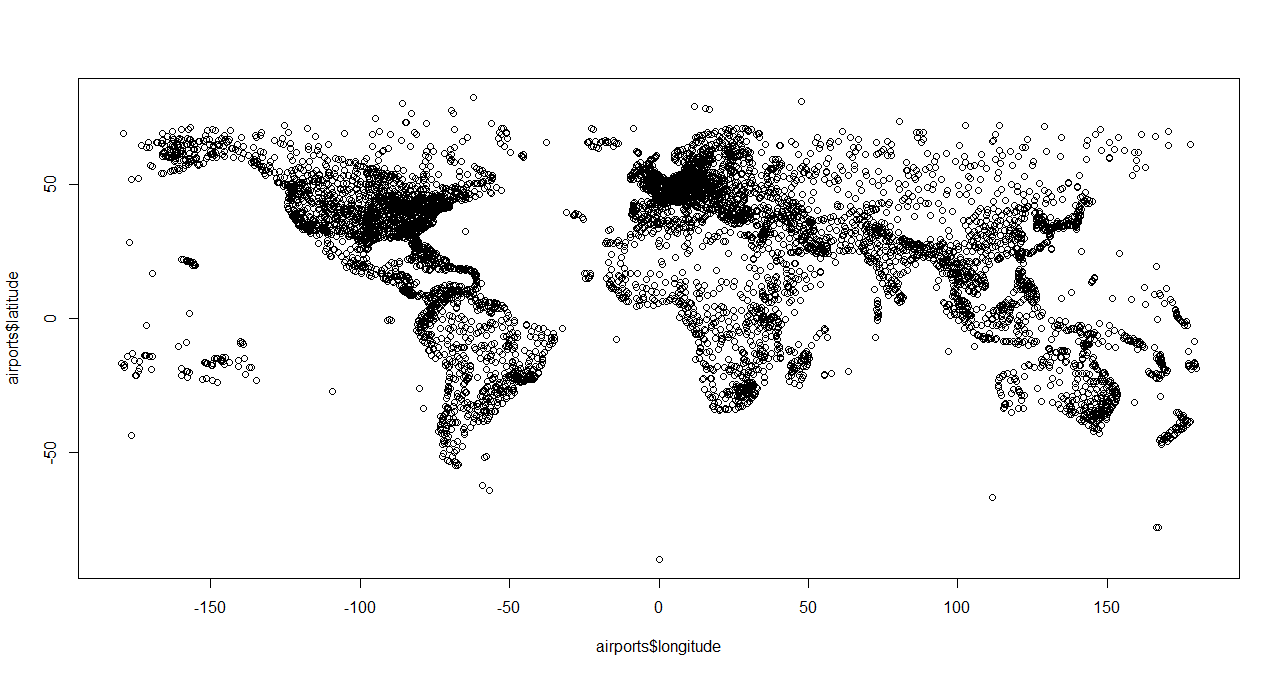
\includegraphics[width=\textwidth, height=\textheight,keepaspectratio]{LonLatMapV1}
	\end{minipage}
	\newline
	\begin{minipage}{\textwidth}
		\centering
		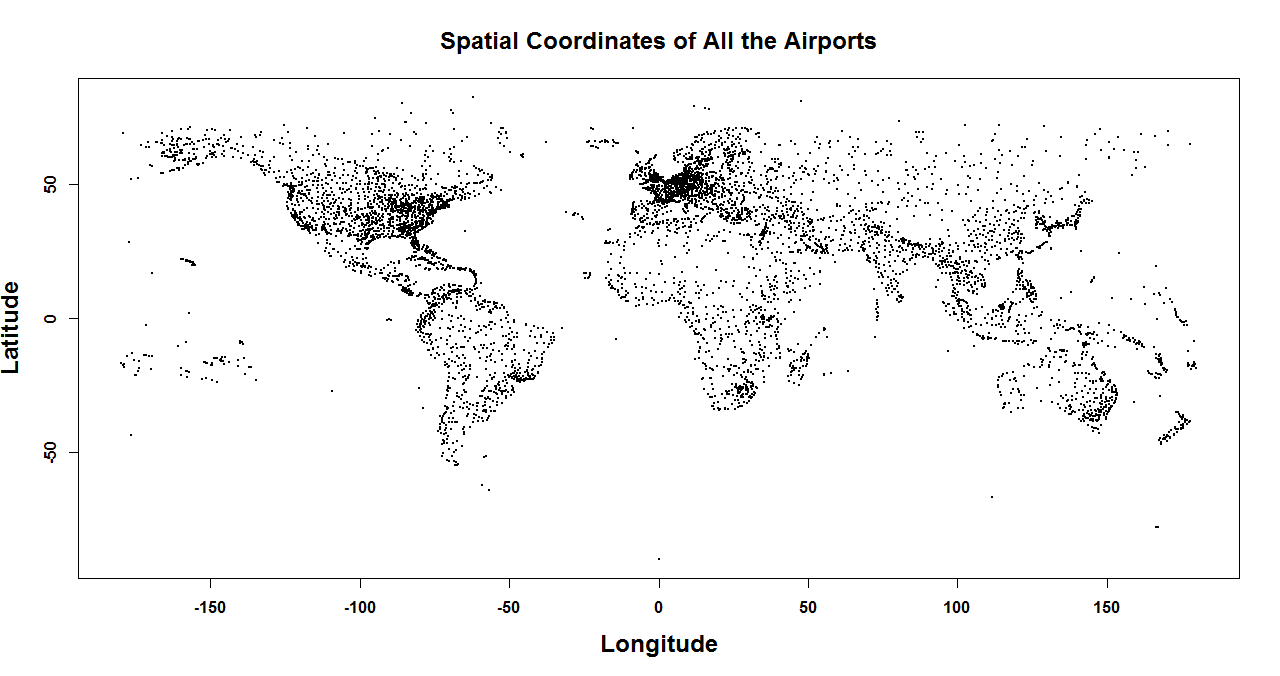
\includegraphics[width=\textwidth, height=\textheight,keepaspectratio]{LonLatMapV2}
	\end{minipage}
	\caption{Passage de paramètres graphiques à la commande \emph{plot}}
\end{figure}
\label{fig:LonLatMap}

\begin{lstlisting}[caption = Utilisation de la commande \emph{plot},label=src:plot]
plot(airports$longitude,airports$latitude)
plot(airports$longitude,airports$latitude,cex = 0.1,xlab="Longitude",ylab="Latitude",main="Spatial Coordinates of All the Airports",pch = 20,font = 2,cex.main = 1.5,font.lab = 2,cex.lab = 1.5)
\end{lstlisting}

\vspace{\baselineskip}
Dans le cas où nous aurions plutôt voulu faire la représentation d'une fonction continue, nous pourrions encore une fois utiliser la commande \emph{plot} en modifiant l'argument \emph{type}. Bien que cette pratique peut nous sembler justifiée, elle pourra jouer de mauvais tours à un utilisateur non averti. Comme le montre la \autoref{fig:plotCurve}, dépendamment de l'espacement des valeurs des points calculés, nous pourrions perdre toute l'information sur l'allure réelle de la courbe que nous cherchons à visualiser. \\

Il sera donc préférable d'utiliser la commande \emph{curve} \cite{Rfunction:curve} pour ce genre de tâche afin de simplifier le code source en ne précisant que les extrêmes de l'étendue sur lequel nous voulons tracer la fonction en spécifiant au besoin le nombre de valeurs à calculer dans l'intervalle. \\

\begin{lstlisting}[caption = Utilisation de la commande \emph{curve},label=src:plotCurve]
fquad <- function(x,a=2,b=3,c=4)
{
  a*x**2+b*x+c
}
fquad(2)
par(mfrow = c(2,2))
plot(x <- seq(-10,10,10),fquad(x,2,3,4),type = "l",ylab = "fquad(x)",xlab = "x",main = "dx = 10")
plot(x <- seq(-10,10,5),fquad(x,2,3,4),type = "l",ylab = "fquad(x)",xlab = "x",main = "dx = 5")
plot(x <- seq(-10,10,2),fquad(x,2,3,4),type = "l",ylab = "fquad(x)",xlab = "x",main = "dx = 2")
plot(x <- seq(-10,10),fquad(x,2,3,4),type = "l",ylab = "fquad(x)",xlab = "x",main = "dx = 1")

par(mfrow = c(1,1))
curve(fquad(x),from = -10,to = 10)
\end{lstlisting}

\addPicture{1}{0.5}{plotCurve}{Tracer une courbe avec la commande \emph{plot}}{plotCurve}

\addPicture{1}{0.5}{curve}{Tracer une courbe avec la commande \emph{curve}}{curve}

\vspace{\baselineskip}
Un autre type de graphique fréquemment utilisé dans les analyses statistiques sont les histogrammes. Ces derniers permettent de rapidement avoir une idée globale sur le type de distribution à laquelle nous sommes confrontés. L'argument \emph{breaks} de la commande \emph{hist} \cite{Rfunction:hist} est de loin le plus important puisqu'il permettra d'obtenir un visuel beaucoup plus précis de la situation en réduisant la taille des regroupements effectués. En ne spécifiant qu'un seul nombre à cet argument, nous indiquons à R de diviser les données pour obtenir ce même nombre de groupes d'étendue équivalente. Dans le cas où un vecteur de nombre lui serait fourni, R comprendra plutôt qu'il doit regrouper les données en utilisant ces nombres à titre de bornes pour les différents intervalles. Un autre argument bien intéressant est \emph{freq}. Cet argument booléen contrôlera l'affichage de la hauteur des colonnes de l'histogramme. Le nombre d'observations sera affiché si sa valeur est vraie (valeur par défaut) ou sous la forme d'une probabilité. \\

\begin{moreInfo}{\emph{Excel} et les histogrammes}
	Si vous êtes habitués de travailler avec \emph{Excel}, vous avez probablement une mauvaise impression de la valeur ajoutée d'utiliser des histogrammes. Ceci vient du fait qu’ \emph{Excel} travaille plutôt avec des graphiques à bâtons. La différence entre ces deux types de graphique réside dans le fait que les colonnes d'un histogramme possèderont à la fois une largeur et une hauteur, tandis que les diagrammes à bâtons ne possèdent qu'une notion de hauteur et sont plutôt destinés à représenter la distribution d'une variable qualitative. 
\end{moreInfo}

La fonction \emph{density} \cite{Rfunction:density} est aussi très intéressante d'un côté pratique pour estimer la fonction de densité empirique sous-jacente. Cette fonction possède un argument \emph{adjust} avec lequel nous contrôlerons le degré de lissage employé. La valeur par défaut de cet argument est 1 et plus sa valeur sera faible, plus nous nous rapprochons de la distribution discrête, tandis qu'une valeur supérieure aura pour effet de lisser davantage la fonction obtenue. \\

Bon nombre des fonctionnalités graphiques de R peuvent être combinées au sein d'un même graphique. Il s'agira d'un comportement natif dans certains cas (les commandes \emph{points} et \emph{lines}) ou d'un comportement induit par l'argument \emph{add} comme c'est possible de le faire avec \emph{curve}. Il sera possible de facilement tracer la fonction de densité renvoyée par \emph{density} grâce à la commande \emph{lines}. \\

La commande \emph{abline} \cite{Rfunction:abline} simplifiera grandement l'affichage de fonctions linéaires. L'utilisation de celle-ci pourra se faire de trois manières différentes. La première consiste à spécifier les arguments \texttt{a} et \texttt{b} pour produire la représentation d'une droite d'équation $y = ax + b$. La deuxième permettra plutôt de tracer une droite d'équation $y = h$ en attribuant une valeur à l'argument \texttt{h}. La dernière et non la moindre qui est, selon moi, la plus commode d'entre toutes permet de créer des droites d'équation $x = v$. L'ajout de ce genre de droites permettra de faire ressortir des valeurs d'abscisses ayant une signification particulière dans le cadre de votre analyse. \\

Certaines autres fonctions vous permettront de rajouter de l'information afin de faciliter la lecture de vos graphiques. Parmi ces fonctions, la plus importante sera \emph{legend} qui comme son nom l'indique, s'occupera de générer une légende au graphique que nous venons de produire. Cette fonction est tout autant paramétrisable que le graphique sous-jacent. Nous pouvons tout de même identifier des arguments plus communs que d'autres. L'argument \emph{bty} permettra de supprimer l'encadrement de la légende en lui attribuant la valeur "n". Nous préciserons aussi un type de points avec \emph{pch} ou un type de ligne avec \emph{lty} sur lesquels nous pourrons affecter la même couleur que la courbe correspondante à l'aide de \emph{col}. La fonction \emph{mtext} s'occupera plutôt d'ajouter du texte à des endroits précis sur le graphique pour noter des observations ou ajouter des explications sur des aspects qui nous semblent plus surprenants. \\

L'ensemble des points discutés ci-dessus ont été repris dans le \autoref{src:histAltitude} pour produire la \autoref{fig:histAltitude}. \\

\begin{lstlisting}[caption = {\emph{hist}, \emph{density}, \emph{lines}, \emph{abline}, \emph{legend} et \emph{mtext}},label=src:histAltitude]
Altitude <- as.numeric(paste(airportsCanada$altitude))
hist(Altitude)
hist(Altitude,xlim = c(0,5000))
hist(Altitude,xlim = c(0,5000),breaks = 100)
hist(Altitude,xlim = c(0,5000),breaks = 100,freq = FALSE,col = "gray",border = grey(0.8),font = 2,font.lab = 2)
lines(density(Altitude,adjust = 4),lwd = 2, col = "blue")
lines(density(Altitude,adjust = 1),lwd = 2, col = "purple")
lines(density(Altitude,adjust = 0.25),lwd = 2, col = "red")
altitudeAvg <- round(mean(Altitude),1)
abline(v = altitudeAvg,lwd = 2)
legend(2500,0.0015,legend = c("4","1","0.25"),title = "Density Adjustment \n Factor",col = c("blue","purple","red"),bty = "n",title.col = "black",lty = 1,lwd = 3,y.intersp = 0.5,cex = 1.25)
mtext(paste("Average: \n",altitudeAvg),at = altitudeAvg,cex = 0.75)
\end{lstlisting}

\addPicture{1}{0.5}{histAltitude}{Distribution des altitudes des aéroports canadiens}{histAltitude}

\begin{moreInfo}{Vers l'infini et plus loin encore!}
	Vous aurez compris qu'il ne s'agit que d'un TRÈS bref aperçu des capacités graphiques de R. Il existe des structures standard pour générer d'autres types de graphique tels que les diagrammes en pointes de tarte (\emph{pie}) ou encore les boîtes à moustaches (\emph{boxplot}). \\
	Certains d'entre vous trouveront peut-être que la génération de graphique est un processus lent et ardu, mais il s'agit ici du coût à payer pour avoir autant de flexibilité. Ces mêmes personnes seront toutefois heureuses d'apprendre que plusieurs paquetages intègrent des modules de visualisation standard pour les objets qui leur sont propres.  Il serait par contre un peu prétentieux de définir et de modifier les options d’affichage par défaut des objets dont l’existence ne dépend aucunement de leur utilisation.
\end{moreInfo}

\section{Outils d'analyse statistique en R}
	Un des aspects du langage R sur lequel sa réputation s'est bâtie est la variété des outils statistiques qu'il place à la disposition de son utilisateur. Sans même avoir à importer une quelconque librairie à partir de CRAN, plusieurs distributions statistiques sont disponibles. La \autoref{tab:distStatsR} fait la revue des ces distributions et de leur identifiant R correspondant. \cite{distStatsR} \\

\begin{table}[h]
	\centering
	\begin{tabular}{cc}
		\textbf{Distribution} & \textbf{identifiant R} \\
		\hline
		Bêta & beta \\
		Binomiale & binom \\
		Binomiale négative & nbinom \\
		Chi Deux & chisq \\
		Exponentielle & exp \\
		Fisher & f \\
		Gamma & gamma \\
		Géometrique & geom \\
		Hypergéometrique & hyper \\
		Normale & norm \\
		Poisson & pois \\
		Student & t \\
		Uniforme & unif \\
		Weibull & weibull	
	\end{tabular}
	\caption{Liste des distributions statistiques disponibles en R}
\end{table}
\label{tab:distStatsR}

D'autres distributions deviendront aussi disponibles via des paquetages dédiés à cette fin. Le paquetage \texttt{actuar} \cite{Rpackage:actuar} donne accès à plusieurs distributions supplémentaires communément utilisées en actuariat. La distribution Pareto en est un bon exemple. \\

Un aspect particulièrement intéressant de ces implémentations de distribution statistique (qu'elles soient disponibles par défaut en R ou via l'importation d'un paquetage) est la constance dans la structure de ces fonctions. Pour chacune des distributions, nous retrouverons en autre les trois fonctions qui suivent: \\

\begin{description}[style=multiline,leftmargin=2cm]
	\item[$d\langle ID_R \rangle$] Calcule la valeur de la fonction de densité de la distribution ayant l'identifiant R $\langle ID_R \rangle$.
	\item[$p\langle ID_R \rangle$] Calcule la valeur de la fonction de répartition de la distribution ayant l'identifiant R $\langle ID_R \rangle$.
	\item[$q\langle ID_R \rangle$] Renvoie le quantile associé à la valeur fournie en argument selon  la fonction de répartition de la distribution ayant l'identifiant R $\langle ID_R \rangle$.
	\item[$r\langle ID_R \rangle$] Permet de générer des valeurs aléatoires suivants la distribution ayant l'identifiant R $\langle ID_R \rangle$.
\end{description}

De plus, les arguments de ces fonctions se présenteront toujours sous le même format. Nous devrons soit fournir la valeur à laquelle nous voulons évaluer la fonction ou encore un nombre d'observations à générer dans le cas des fonctions préfixées par "r" et les paramètres de la loi utilisée. À des fins d'optimisation des performances, le logarithme de ces fonctions sera souvent nécessaire et c'est ce qui explique la présence de l'argument \texttt{log}. \footnote{Plusieurs propriétés statistiques découlent du logarithme des fonctions de densité et de répartition tel que la fonction génératrice de moments pour ne nommer que cette denière.} Finalement, nous serons parfois intéressés par la fonction de survie d'une distribution donnée correspondant au complément de la fonction de répartition. En attribuant la valeur \textit{FALSE} à l'argument \texttt{lower.tail}, les fonctions préfixées par "p" renverront ainsi la valeur de la fonction de survie. Un exemple d'utilisation de ces fonctions est présenté par le \autoref{src:distStats}. \\

\begin{lstlisting}[caption = Fonctions relatives à la distribution Normale,label=src:distStats]
> set.seed(2017)
> mean <- 6
> sd <- 2
> x <- 0:12
> dnorm(x,mean,sd)
 [1] 0.002215924 0.008764150 0.026995483 0.064758798
 [5] 0.120985362 0.176032663 0.199471140 0.176032663
 [9] 0.120985362 0.064758798 0.026995483 0.008764150
[13] 0.002215924
> pnorm(x,mean,sd)
 [1] 0.001349898 0.006209665 0.022750132 0.066807201
 [5] 0.158655254 0.308537539 0.500000000 0.691462461
 [9] 0.841344746 0.933192799 0.977249868 0.993790335
[13] 0.998650102
> r <- seq(0,1,0.1)
> qnorm(r,mean,sd)
 [1]     -Inf 3.436897 4.316758 4.951199 5.493306
 [6] 6.000000 6.506694 7.048801 7.683242 8.563103
[11]      Inf
> rnorm(10,mean,sd)
 [1] 8.868403 5.845416 7.478274 2.482791 5.860350
 [6] 6.903811 2.083267 5.996951 5.469328 9.126445
\end{lstlisting}

Ceux qui sont familiers avec les distributions statistiques auront remarqué qu'à l'aide des fonctions décrites ci-dessus nous aurons donc deux manières de générer des nombres aléatoires. La première qui est aussi la plus évidente sera d'utiliser les fonctions préfixées avec "r". La seconde utilisera le théroême de la réciproque consistant à générer des valeurs aléatoires suivant une loi uniforme de paramètre $a := 0$ et $b := 1$ pour ensuite trouver le quantile correspondant de la fonction de répartition de la loi pour laquelle nous voulons générer des nombres aléatoires grâce aux fonctions préfixées par "q". Ces deux techniques sont mises à profit dans le \autoref{src:aleaNorm}. \\

\begin{lstlisting}[caption = Génération de nombres aléatoires,label=src:aleaNorm]
> y1 <- rnorm(1000,mean,sd)
> summary(y1)
    Min.  1st Qu.   Median     Mean  3rd Qu.     Max. 
 0.07041  4.70800  6.02800  6.06200  7.35500 12.59000 
> sd(y1)
[1] 1.96455
> r <- runif(1000)
> y2 <- qnorm(r,mean,sd)
> summary(y2)
   Min. 1st Qu.  Median    Mean 3rd Qu.    Max. 
-0.1347  4.7670  6.0830  6.0910  7.5070 12.2400 
> sd(y2)
[1] 1.966951
\end{lstlisting}

\begin{moreInfo}{Théorème de la réciproque}
	Ce sont les 4 propriétés des fonctions de répartition qui rendent possible l'application du théorème de la réciproque. Ces propriétés sont définies comme suit (où $F$ désigne la fonction de répartition d'une variable aléatoire $X$ quelconque):
	\begin{enumerate}
		\item $F_X$ est croissante
		\item Elle est partout continue à droite
		\item $lim_{x \rightarrow -\infty} F_X(x) = 0$
		\item $lim_{x \rightarrow \infty} F_X(x) = 1$
	\end{enumerate}
	Étant donné que ces propriétés seront toujours respectées pour toute fonction de répartition, nous pourrons appliquer cette méthode, peu importe la distribution qu'elle soit clairement définie ou non! \\
	\url{https://fr.wikipedia.org/wiki/Fonction_de_r%C3%A9partition#Th.C3.A9or.C3.A8me_de_la_r.C3.A9ciproque}
\end{moreInfo}

En présence de données empiriques, la première étape d'une analyse statistique sera de dresser le portrait statistique de ces données. Nous avons déjà parlé de la fonction \texttt{summary} à la \autoref{subsec:extraction}. Nous rajouterons ici les fonctions \texttt{mean} et \texttt{sd} retournant respectivement la moyenne et l'écart-type d'un jeu de données empiriques comme nous l'avons fait montré dans le \autoref{src:aleaNorm}. \\

Afin de valider l'ajustement d'une distribution sur les données empiriques, nous serons souvent contraints à identifier les fonctions de densité et de répartition sous-jacentes. Il existe plusieurs façons de faire. Celle qui nous semble toutefois la plus pertinente et polyvalente exploite le comportement de la fonction \texttt{ecdf}. Cette dernière permet de construire une fonction de répartition empirique à partir des observations fournies en argument. Nous pouvons ensuite construire une fonction de densité empirique en évaluant cette fonction de répartition à deux points autour de la valeur désirée et en divisant ensuite le résultat par la largeur de l'intervalle évalué. Les instructions permettant de construire ces fonctions sont fournies par \autoref{src:fctEmp}. \\

\begin{lstlisting}[caption = Fonctions de densité et de répartition empiriques,label=src:fctEmp]
empCDF <- ecdf(compData$weight)
empPDF <- function(x,delta=0.01)
{
  (empCDF(x+delta/2)-empCDF(x-delta/2))/delta
}
\end{lstlisting}

\vspace{\baselineskip}
En plus de dresser le portrait statistique des données, on peut aussi vouloir faire des tests statistiques à partir de celles-ci. Parmi les tests disponibles, nous retrouvons notamment :
\begin{itemize}
	\item Test de normalité (Test de Shapiro-Wilk)
	\item Test de comparaison de deux variances (Test F)
	\item Test de Student
	\item Test du Khi carré
	\item Test de Wilcoxon
	\item ANOVA (Analyse de variance)
	\item Test de corrélation
\end{itemize}
Il n'est toutefois pas indispensable de connaître l'utilité de tous ces tests, les situations dans lesquelles ils devront être utilisés ni la mécanique mathématique sous-entendue puisque la plupart des méthodes statistiques incluront déjà les appels nécessaires de ceux-ci. Ce sera le cas de la fonction \texttt{lm} comme nous le verrons plus loin. \cite{testStatsR} \\

Dans le cadre de notre étude de cas, nous avons performé les tests du Khi carré et de corrélation afin de s'assurer que les variables explicatives du poids et de la distance soient indépendantes et sans corrélation. Dans le cas où ce genre de phénomène serait apparu entre nos variables, nous aurions été contraints d'utiliser des modèles de régression plus complexes tels que les modèles linéaires généralisés. \\

Lorsque nous effectuons un test statistique, nous cherchons toujours à répondre à une question binaire représentée sous la forme de deux hypothèses $H_0$ et $H_1$ complémentaires. Une valeur nommée la \texttt{p-value} sera ensuite calculée en acceptant l'hypothèse $H_0$ comme vraie. Cette valeur correspondra à la probabilité d'observer un résultat équivalent ou supérieur du test que nous venons d'exécuter en considérant l'hypothèse nulle comme vraie. En d'autres mots, cette valeur nous indiquera la probabilité de se tromper en rejetant l'hypothèse nulle en considérant l'hypothèse nulle comme vraie initialement. Ainsi, à partir du moment où la \texttt{p-value} sera inférieure au seuil de crédibilité que l'on s'était fixé (habituellement 5\%), nous considérerons l'hypothèse nulle comme fausse. \\ 

Dans le cas du test du Khi carré, l'hypothèse nulle suppose que les deux distributions sont indépendantes. Le test de corrélation suppose tant qu'à lui que la valeur théorique de corrélation est équivalente à 0. Comme nous pouvons le voir avec le \autoref{src:testStat}, nous ne pouvons pas rejeter ces deux hypothèses. \\

\begin{lstlisting}[caption = Tests d'indépendance et de corrélation entre distributions,label=src:testStat]
> weightsBinded <- as.numeric(cut(compData$weight,25))
> distancesBinded <- as.numeric(cut(compData$distance,25))
> contingencyTable <- table(weightsBinded,distancesBinded)
> chisq.test(contingencyTable)

	Pearson's Chi-squared test

data:  contingencyTable
X-squared = 248.38, df = 391, p-value = 1

Warning message:
In chisq.test(contingencyTable) :
  Chi-squared approximation may be incorrect
> contingencyTable <- rbind(contingencyTable[1:4,],colSums(contingencyTable[5:18,]))
> contingencyTable <- cbind(contingencyTable[,1:14],rowSums(contingencyTable[,15:24]))
> (independencyTest <- chisq.test(contingencyTable))

	Pearson's Chi-squared test

data:  contingencyTable
X-squared = 72.814, df = 56, p-value = 0.06495

> cor.test(compData$weight,compData$distance,method = "pearson")

	Pearson's product-moment correlation

data:  compData$weight and compData$distance
t = -0.7801, df = 99998, p-value = 0.4353
alternative hypothesis: true correlation is not equal to 0
95 percent confidence interval:
 -0.008664731  0.003731121
sample estimates:
       cor 
-0.0024669 
\end{lstlisting}

\vspace{\baselineskip}
Il est pertinent de remarquer que le test du Khi carré possède des limitations importantes dans le cas de distributions devenant un peu trop clairsemées. Ce test nécessite une efficience statistique d'au minimum 5 observations à toutes les intersections des deux variables catégoriques. C'est pour cette même raison que nous combinons les dernières lignes et colonnes de la table de contingence. Malgré tout, le test offre toujours une \texttt{p-value} d'environ 6\% ce qui reste supérieur à notre seuil de 5\% et nous ne pouvons donc pas rejeter notre hypothèse nulle. Dans le cas du test de corrélation, nous voyons que la valeur 0 est comprise dans notre intervalle de confiance autour de la valeur de corrélation empirique déterminée, ce qui nous permet d'affirmer qu'aucune corrélation n'existe entre ces deux variables. La \texttt{p-value} de 43\% aurait été suffisante pour arriver à la même conclusion. \\

Pour terminer cette section, jetons un coup d'oeil à la régression linéaire qui fut accomplie dans le but de modéliser la distribution ayant mené à générer les données (\autoref{src:linReg}).

\begin{lstlisting}[caption = Régression linéaire sur données empiriques,label=src:linReg]
> profitMargin <- 1.12
> avgTaxRate <- sum(table(airportsCanada$province)*as.numeric(paste(taxRates$taxRate)))/length(airportsCanada$province)
> compModel <- lm(price/(profitMargin*avgTaxRate) ~ distance + weight, compData)
> summary(compModel)

Call:
lm(formula = price/(profitMargin * avgTaxRate) ~ distance + weight, 
    data = compData)

Residuals:
     Min       1Q   Median       3Q      Max 
-30.7903  -4.6585   0.0305   4.6462  29.9563 

Coefficients:
             Estimate Std. Error t value Pr(>|t|)    
(Intercept) 3.227e+01  7.509e-02   429.7   <2e-16 ***
distance    2.820e-02  9.206e-05   306.4   <2e-16 ***
weight      7.252e-01  9.479e-03    76.5   <2e-16 ***
---
Signif. codes:  
0 '***' 0.001 '**' 0.01 '*' 0.05 '.' 0.1 ' ' 1

Residual standard error: 6.89 on 99997 degrees of freedom
Multiple R-squared:  0.499,	Adjusted R-squared:  0.499 
F-statistic: 4.98e+04 on 2 and 99997 DF,  p-value: < 2.2e-16
\end{lstlisting}

\vspace{\baselineskip}
L'appel de la fonction \texttt{lm} \cite{Rfunction:lm} est assez rudimentaire. Il suffit de fournir une formule de régression contenant les variables explicatives avec lesquelles nous tenons à faire la régression et nous spécifions le nom de la table contenant ces variables. Nous remarquons ici la technique du retour multiple abordée à la \autoref{sec:fctUtil}. Nous voyons aussi que pour chaque coefficient un test de Student a été effectué pour déterminer à quel point l'estimation était significativement différente de 0. D'autre part, le test de Fisher permet de savoir s'il existe réellement une relation entre les variables explicatives choisies et la variable réponse analysée. \cite{outputLM} \\

Lorsque l'on compare les valeurs réellement utilisées dans le \autoref{src:Benchmark} et les coefficients estimés, nous voyons que ces derniers sont très proches les uns des autres. La \autoref{tab:linRegFit} fait la revue de ces valeurs. \\

\begin{table}[h]
	\centering
	\begin{tabular}{ccc}
		\textbf{Variable} & \textbf{Valleur réelle} & \textbf{Valeur estimée} \\
		\hline
		distance & 0.0275 & 0.0282 \\
		poids & 0.7 & 0.7252		
	\end{tabular}
	\caption{Comparaison entre les coefficients réels et estimés par régression linéaire}
	\label{tab:linRegFit}
\end{table}

\begin{moreInfo}{Lire des tables directement sur le web}
	Afin de récupérer les valeurs sur les niveaux de taxe pour chaque province canadienne, nous avons pris l'initiative de passer directement via le web. Cette méthode possède l'avantage de se mettre à jour directement avec l'information la plus récente si la structure de la page n'est pas modifiée. Afin de parvenir à ce résultat, les paquetages \texttt{XML}, \texttt{RCurl} et \texttt{rlist} fournissent des fonctions permettant d'interpréter la structure \texttt{HTML} d'une page web spécifiée par le passage du chemin \texttt{url} en argument à la fonction \texttt{readHTMLTable} pour y détecter les occurrences de balises du genre $\langle table \rangle$, $\langle tr \rangle$, $\langle th \rangle$ et $\langle td \rangle$.  $$\langle table \rangle \langle td \rangle \dots \langle /td \rangle \langle /table \rangle$$.
	\url{http://web.mit.edu/~r/current/arch/i386_linux26/lib/R/library/XML/html/readHTMLTable.html}
\end{moreInfo}

	\label{sec:statsTools}

\section{Ajustement de distributions statistiques sur données empiriques}
	En plus des capacités statistiques impressionnantes que nous avons survolées à la section précédente, R dispose d'une vaste gamme d'outils d'optimisation. Pour ne pas trop nous écarter du but premier de cette documentation, soit de faire une revue globale des fonctionnalités de R en utilisant une étude de cas à titre de support de présentation, nous concentrerons la discussion autour des fonctions \texttt{optim} \cite{Rfunction:optim} et \texttt{fitdistr} \cite{Rfunction:fitdistr}. Nous terminerons en présentant comment répliquer le comportement de la fonction \texttt{fitdistr} dans le cadre d'une fonction utilitaire. \\

La fonction \texttt{optim} est un excellent choix de fonction pour aborder tout problème d'optimisation. Contrairement à bien d'autres outils, cette fonction permettra d'optimiser plusieurs paramètres à la fois. Elle imposera tout de même quelques limitations telles que l'impossibilité de facilement préciser un intervalle d'optimisation, le fait qu'elle ne pourra que minimiser la fonction étudiée et l'obligation de lui fournir des valeurs de départ. \cite{optim} \\

Parmi les arguments de la fonction \texttt{optim}, nous devrons minimalement désigner les valeurs de départ de nos paramètres avec \texttt{par} \footnote{À ne pas confondre avec la fonction permettant de contrôler l'affichage graphique \texttt{par}.} et fournir à \texttt{fn} la fonction à minimiser. Il sera possible de définir des bornes aux valeurs optimisées grâce aux arguments \texttt{lower} et \texttt{upper}. Le \autoref{src:optim} illustre une application standard de cette fonction. Vous ne serez pas surpris de rencontrer à nouveau la technique du retour multiple au sein d'une liste. De cette liste, nous utiliserons principalement les attributs \texttt{par} et \texttt{value}. Ceux-ci nous donneront accès aux paramètres optimisés et à la valeur de convergence obtenue. Il sera conseillé de garder un oeil sur \texttt{convergence} qui indiquera si l'optimisation s'est terminée de manière conforme (valeur de 0) ou que le processus d'optimisation  n’est pas parvenu à converger (valeur de 1). La valeur de \texttt{counts} témoigne du nombre d'itérations effectuées afin d'arriver aux résultats. Par défaut, la fonction \texttt{optim} arrêtera au compte de 501 itérations après quoi les valeurs actuelles de l'optimisation seront renvoyées en plaçant toutefois la valeur de l'attribut \texttt{convergence} à 1. \\

\begin{lstlisting}[caption = Optimisation générique avec R,label=src:optim]
> f1 <- function(x,y) 5*x**2 - 7*y + 10
> f2 <- function(x,y) 10*x**2 + 30*y -2
> foptim <- function(x1,x2) (f1(x1,x2) - f2(x1,x2))**2
> (results <- optim(par = c(4,5), function(par) foptim(par[1],par[2])))
$par
[1] 0.4532121 0.2968149

$value
[1] 8.385268e-05

$counts
function gradient 
      57       NA 

$convergence
[1] 0

$message
NULL

> f1(results$par[1],results$par[2])
[1] 8.949302
> f2(results$par[1],results$par[2])
[1] 8.958459
\end{lstlisting}

\vspace{\baselineskip}
Malgré le fait que nous ayons mentionné des limitations à la fonction \texttt{optim}, cela ne signifie pas pour autant que nous ne pourrons pas imaginer des manières de contourner ces dernières. En effet, une maximisation revient tout simplement à trouver la valeur minimale de l'inverse de la fonction étudiée. Ainsi, le simple ajout d'un signe de négation devant la fonction passée à l'argument \texttt{fn} nous permettra d'effectuer une maximisation plutôt qu'une minimisation. Il s'agit là de la stratégie employée dans le \autoref{src:optimMax}. \\

Il n’est pas rare que plus d’une solution soit viable aux yeux d’un processus d’optimisation dépendamment du problème étudié. Nous appelons ces nombreuses solutions des extremums locaux. C'est l'existence de ces extremums qui rend les valeurs initiales de l'optimisation si sensibles. Lorsque possible, il sera donc fortement conseillé de procéder à des techniques de validation graphique comme nous l'avons fait dans le cadre du \autoref{src:optimMax}. (Voir \autoref{fig:optimMax}) \\

\begin{lstlisting}[caption = Maximisation d'une fonction avec \texttt{optim},label=src:optimMax]
> f3 <- function(x,y) -x**2 - 2*y**2 + 3*x + 4*y - 5
> (results <- optim(par = c(0,0), function(par) -f3(par[1],par[2])))
$par
[1] 1.5001064 0.9999031

$value
[1] 0.75

$counts
function gradient 
      69       NA 

$convergence
[1] 0

$message
NULL

> # install.packages("rgl")
> library(rgl)
> persp3d(f3,xlim = c(-5,5),ylim = c(-5,5))
\end{lstlisting}

\addPicture{1}{0.5}{optim3d}{Représentation graphique de la fonction \texttt{f3}}{optimMax}

\begin{moreInfo}{Contrôler l'incontrôlable}
	Bien que vous n'aurez pas à modifier le comportement par défaut de la fonction \texttt{optim} pour parvenir à vos fins, il est important de savoir que la fonction propose plusieurs arguments qui permettent d'influencer la manière par laquelle l'optimisation sera effectuée. Nous pouvons rapidement citer les arguments \texttt{method} et \texttt{control}. Veillez vous référer à la documentation officielle pour de plus amples détails à leur sujet. \\
	\url{https://stat.ethz.ch/R-manual/R-devel/library/stats/html/optim.html}
\end{moreInfo}

Une autre fonction d'intérêt lorsque nous travaillons avec des distributions statistiques est \texttt{fitdistr} provenant du paquetage \texttt{MASS}. Celle-ci permet de facilement ajuster une distribution donnée à un jeu de données empiriques. Évidemment, nous pourrions très bien passer par \texttt{optim} pour réaliser le même travail moyennant un certain coût de complexité. Or, ce mal sera parfois nécessaire puisque la fonction \texttt{fitdistr} n'est définie que pour les distributions suivantes : \cite{MASS}

\begin{minipage}{\linewidth}
	\begin{multicols}{2}
		\begin{itemize}
			\item Bêta
			\item Binomiale négative
			\item Cauchy
			\item Khi carrée
			\item Exponentielle
			\item F (Fisher)
			\item Gamma
			\columnbreak
			\item Géometrique
			\item Log-Normale
			\item Logistique
			\item Normale
			\item Poisson
			\item T (Student)
			\item Weibull
		\end{itemize}
	\end{multicols}
\end{minipage}
\vspace{\baselineskip}

Il arrivera donc dans certains cas que nous devrons procéder à l'ajustement des distributions par la méthode du maximum de vraisemblance directement avec \texttt{optim}. Nous prioriserons toutefois l'utilisation de \texttt{fitdistr}. \\

L'appel de \texttt{fitdistr} se fera la majorité du temps en passant un vecteur de données sur lesquelles ajuster la distribution et en précisant le nom de la distribution à ajuster. Ce qui présente un net avantage en terme de simpliciter par rapport à l'appel de la fonction \texttt{optim} qui permettra d'accomplir le même travail. Le \autoref{src:fitdistr} présente l'utilisation de ces deux méthodes. \\

\begin{lstlisting}[caption = Ajustement de distribution sur données empiriques,label=src:fitdistr]
> x <- rgamma(1000,40,3)
> optim(c(10,1),function(par) -sum(dgamma(x,par[1],par[2],log = TRUE)))
$par
[1] 37.216936  2.785522

$value
[1] 2193.865

$counts
function gradient 
      69       NA 

$convergence
[1] 0

$message
NULL

> #install.packages("MASS")
> library(MASS)
> fitdistr(x,"gamma")
     shape         rate   
  37.1275898    2.7787518 
 ( 1.6529478) ( 0.1245497)
\end{lstlisting}

Les mordus de statistiques parmi vous auront constaté que les distributions reconnues par \texttt{fitdistr} ne nécessitent pas toujours le même nombre de paramètres. Il s'agit là d'une complexité algorithmique de bonne taille. Dans le cadre de l'étude de cas, nous avons cru bon de créer une réplique de cette fonction afin d'expliquer comment nous pouvons nous y prendre pour créer des fonctions aussi flexibles. Voici pour commencer le code source de cette fameuse fonction : \\

\begin{lstlisting}[caption = Réplicat maison de la fonction \texttt{fitdistr} ,label=src:distFit]
#' Generic function for statistical distribution adjustment
#' 
#' @param data A vector of value over which we want to fit the distribution
#' @param dist The distribution name
#' @param ... The initial values to be given to the optimisation function
#' @return A list containing : 
#' the optimized parameters, 
#' the error value, 
#' the deviance measure,
#' the convergence indicator and 
#' the number of iterations necessited
#' @examples
#' x <- rnorm(1000,10,2)
#' distFit(x,"Normal", 1, 1)
#' x <- rgamma(1000,5,1)
#' distFit(x,"Gamma", 1, 1)
#' 
distFit <- function(data,dist,...)
{
  dist = tolower(dist)
  args = list(...)
  if(dist == "normal")
  {
    law = "norm"
    nbparam = 2
  }
  else if(dist == "exp")
  {
    law = "exp"
    nbparam = 1
    lower = 0
    upper = 100/mean(data)
  }
  else if(dist == "gamma")
  {
    law = "gamma"
    nbparam = 2
  }
  else if(dist == "lognormal")
  {
    law = "lnorm"
    nbparam = 2
  }
  else if(dist == "weibull")
  {
    law = "weibull"
    nbparam = 2
  }
  else if(dist == "pareto")
  {
    law = "pareto"
    nbparam = 2
  }
  else if(dist == "invgaussian")
  {
    law = "invgauss"
    nbparam = 2
  }
  else if(dist == "student")
  {
    law = "t"
    nbparam = 1
    lower = 0
    upper = 100/mean(data)
  }
  else if(dist == "burr")
  {
    law = "burr"
    nbparam = 3
  }
  else
  {
    message <- "The only distributions available are: 
    Normal, Exp, Gamma, LogNormal, Weibull, Pareto, Student, Burr and InvGaussian.
    (This case will be ignored)"
    stop(message)
  }
  if(nbparam != length(args))
  {
    message <- paste("There is a mismatch between the number of arguments passed to the 
                     function and the number of arguments needed to the distribution.",
                     "The",dist,"distribution is taking",nbparam,"parameters and",
                     length(args),"parameters were given.")
    stop(message)
  }

  # Treament
  if(nbparam == 1)
  {
    param <- optim(par = args, function(par) 
      -sum(do.call(eval(parse(text = paste("d",law,sep=""))),c(list(data),par,log = TRUE))),
      method = "Brent", lower = lower, upper = upper)
  }
  else{
    param <- optim(par = args, function(par) 
      -sum(do.call(eval(parse(text = paste("d",law,sep=""))),c(list(data),par,log = TRUE))))
  }
  # Deviance value
  devValue <- sum((empPDF(x <- seq(0,max(data),0.1))-do.call(eval(parse(text = paste("d",law,sep=""))),c(list(x),param$par)))**2)
  
  # Return List
  distFitList <- list() 
  distFitList$param <- param$par
  distFitList$errorValue <- param$value
  distFitList$devValue <- devValue
  distFitList$convergence <- param$convergence
  distFitList$nbiter <- param$counts[1]
  distFitList
}
\end{lstlisting}

Le \autoref{src:distFit} peut sembler impressionnant à première vue, mais environ 90\% de son corps ne sert qu'à faire de la gestion d'erreurs. Comme indiqué par les commentaires internes, les lignes de commandes renfermant le secret de ce type de fonction sont les suivantes: \\

\begin{minipage}{\linewidth}
	\noindent
	\texttt{param <- optim(par = args, function(par) -sum(do.call(eval(parse(text = paste("d",law,sep=""))),c(list(data),par,log = TRUE))))}
\end{minipage}

\vspace{\baselineskip}
Sans trop de précisions, la fonction \texttt{parse} permettra de créer des expressions non-évaluées. Il existe plusieurs manières de générer ces expressions. Celle employée dans le cas présent se fera à partir d'un vecteur de caractères qui nous permettra de concaténer le "d" de la fonction de densité à l'identifiant R de la distribution choisie. (Voir \autoref{tab:distStatsR} $\langle ID_R \rangle$) Une fois cette expression construite, nous pourrons la faire évaluer par R grâce à la fonction \texttt{eval} qui transformera la ligne de code en un objet (étant ici la fonction de densité de la distribution choisie). À cet objet, nous pourrons désormais lui fournir des paramètres au même titre que nous le ferions avec la fonction de densité correspondante. Alors pourquoi avons-nous senti le besoin d'utiliser \texttt{do.call}? La fonction \texttt{do.call} rend possible l'appel d'une fonction ayant un nombre d'arguments quelconque. Elle s'occupera de fournir une liste de paramètres à la fonction considérée pour autant que la fonction réceptrice accepte autant d'arguments que fournis et que les types correspondent. Étant donné que le nombre de paramètres de nos distributions peut varier, nous n'aurions pas pu envisager de créer un traitement particulier pour tous les cas possibles.

\begin{lstlisting}[caption = Exemple d'utilisation de la fonction \texttt{distFit},label=src:distFitEx]
> x <- rexp(10000,4)
> distFit(x,"Exp",1)$param
[1] 4.102991
> x <- rt(10000,5)
> distFit(x,"Student",1)$param
[1] 5.056508
> x <- rgamma(10000,4,2)
> distFit(x,"Gamma",1,1)$param
[1] 3.982845 1.981206
> x <- rburr(10000,1,10,0.01)
> distFit(x,"Burr",0.9,1,0.1)$param
[1]  0.95531981 10.09683646  0.01006351
Warning messages:
1: In (function (x, shape1, shape2, rate = 1, scale = 1/rate, log = FALSE)  :
  NaNs produced
2: In (function (x, shape1, shape2, rate = 1, scale = 1/rate, log = FALSE)  :
  NaNs produced
3: In (function (x, shape1, shape2, rate = 1, scale = 1/rate, log = FALSE)  :
  NaNs produced
4: In (function (x, shape1, shape2, rate = 1, scale = 1/rate, log = FALSE)  :
  NaNs produced
\end{lstlisting}

Comme nous venons de le voir, la combinaison de ces trois fonctions ouvre les portes à un autre niveau de flexibilité pour la définition de fonctions utilitaires. Grâce à cet exemple, nous comprenons désormais un peu mieux la mécanique sous-entendue par le passage de paramètres additionnels via l'argument \texttt{(...)}.
	\label{sec:fitDist}

\section{Analyse par simulation en R}
	Quand bien même que la génération de nombres aléatoires ai déjà été abordée à la \autoref{sec:statsTools}, il serait incorrect de s'simaginer que les capacités statistiques de R s'arrête là. R est un excellent langage pour faire du calcul stochastique. Qui dit calcul stochastique dit aussi estimation par simulation d'un grand nombre d'observations pour estimer le comportement d'un phénomène difficilement quantifiable de manière déterministe. \\

La première fonction à connaître lorsque nous abordons une analyse de ce genre est la fonction \texttt{sample}. Cette dernière sera utile dans les cas où nous cherchons à faire une pige aléatoire de taille quelconque (\texttt{size}) sur un ensemble de valeurs fourni par un vecteur. Il sera possible de préciser si nous voulons faire une pige avec ou sans remise avec l'argument \texttt{replace} ainsi la probabilité que chaque valeur survienne grâce à \texttt{prob}. Un aspect fort intéressant de cette fonction et sa capacité de faire des piges sur des valeurs textuelles. Le \autoref{src:sample} fait une revue de l'utilisation de la fonction \texttt{sample}. Lors deux deuxième appel de la fonction, nous remarquons la génértion de valeurs beaucoup plus élevées par rapport au premier appel. Toutefois, la seule différence a été de modifier la valeur de l'argument \texttt{prob} pour y assigner le poids relatif de l'altitude sur l'ensemble des altitudes favorisant ainsi les valeurs plus extrêmes. Le troisième appel expose, quant à lui, la capacité de travailler avec un vecteur de valeurs textuelles. \\

\begin{lstlisting}[caption = Pige aléatoire sur support vectoriel,label=src:sample]
> sample(airportsCanada$altitude,size = 10, replace = TRUE)
 [1] 1211   24 1215 2351 1873  882  256 2314 2968  728
> probs = airportsCanada$altitude/sum(airportsCanada$altitude)
> sample(airportsCanada$altitude,size = 10, replace = TRUE,prob = probs)
 [1] 2525 2264 2680 1220 1087 2277 4296 1536 1712 2000
> sample(unique(as.character(paste(airportsCanada$name))),size = 10,replace = FALSE)
 [1] "Fort Severn Airport"                        
 [2] "CFB Trenton"                                
 [3] "Waterville / Kings County Municipal Airport"
 [4] "Salluit Airport"                            
 [5] "Forestville Airport"                        
 [6] "Taloyoak Airport"                           
 [7] "Sandspit Airport"                           
 [8] "Mary's Harbour Airport"                     
 [9] "Pukatawagan Airport"                        
[10] "Deer Lake Airport"
\end{lstlisting}

En inspectant le \autoref{src:CaseStudyDevQ6}, nous constatons la structure fonctionnelle et imbriquée du processus entrepris. Il sera fortement conseillé de procéder ainsi pour différentes raisons:

\begin{itemize}
	\item Augmenter la clareté du processus de simulation
	\item Faciliter le débogage lors du développement
	\item Possibilité de facilement ajouter et retirer des blocs au casse-tête de simulation
	\item Identification simplifiée des parties limitantes et coûteuses en temps de calcul pour des fins d'optimisation
	\item Permettre la production d'une nouvelle itération par l'appel d'une fonction mère possédant idéalement aucun argument
\end{itemize}

Ce ne sera qu'en présence de cette structure que la fonction \texttt{replicate} prendra tout son sens. À l'aide de cette fonction, nous pourrons commodément contrôler le nombre de répliques effecutées. Dans le \autoref{src:replicate}, nous avons justement pris cette fonctionnalité pour reproduire à 6 reprises la génération de nombres aléatoires suivant une loi $Norm(\mu := 3, \sigma := 4)$.

\begin{lstlisting}[caption = Replication d'une analyse stochastique,label=src:replicate]
fsimul <- function() qnorm(runif(100),3,4)
results <- replicate(6,fsimul())
g <- rep(c("a", "b","c","d","e","f"), each = 100)
#install.packages("lattice")
library(lattice)
histogram(~ as.vector(results) | g,xlab = "Results",ylab = "Frequency") 
\end{lstlisting}

\addPicture{1}{0.5}{replicate}{Comparaison des résultats d'une analyse stochastique à 6 réplicats}{replicate}

\begin{moreInfo}{Une "Poisson" dans une pisciculture...}
	La distribution Poisson sera souvent à la base des processus stochastiques en raison de ses propriétés particulières. Nous parlerons souvent du fait que cette loi ne possède pas de mémoire ce qui implique que le nombre de succès observés sur différents intervalles seront indépendants. Nous pouvons aussi mentionné que la somme des variables aléatoires suivant des lois Poisson indépendantes de paramètres $\lambda_1$ et $\lambda_2$ suivra à son tour une loi de Poisson de paramètre $\lambda_1 + \lambda_2$. \\
	\url{https://ocw.mit.edu/courses/electrical-engineering-and-computer-science/6-262-discrete-stochastic-processes-spring-2011/course-notes/MIT6_262S11_chap02.pdf} \\
	\url{https://fr.wikipedia.org/wiki/Loi_de_Poisson}
\end{moreInfo}
	\label{sec:simul}
	
\chapter*{Conclusion}
	Au terme de cette étude de cas, nous avons su intégrer différentes notions relatives à la programmation en R. Nous avons abordé des sujets aussi variés qu'actuels allant de l'importation des données jusqu'à la simulation stochastique. \\

Cette formation n'a jamais eu la prétention de pouvoir vous apprendre toutes les particularités du langage R ni même faire de vous des programmeurs parfaitement fonctionnels au terme de sa lecture. Par contre, nous croyons avoir bel et bien accompli l'objectif principal qui était de faire une revue des capacités de R tout en vous offrant un coffre d'outils qui facilitera grandement vos débuts avec ce langage de programmation. Il n'y a pas de secret pour apprendre à programmer, mais il existe certainement des moyens plus simples que d'autres. Selon nous, une connaissance adéquate de ce que l'on peut ou pas réaliser consiste un excellent point de départ. Par après, à un moment ou un autre, vous serez confronté à un problème qui vous semblera parfaitement adapté à l'utilisation d'un outil donné. Vous chercherez ensuite à accumuler les ressources nécessaires à sa résolution. Évidemmemnt, rien ne vous empêche de vous créer des problèmes fictifs comme nous l'avons fait pour ensuite lire plusieurs centaines de pages de documentation pour finalement arriver à vos fins. La route sera souvent tortueuse, mais le résultat donc bien satisfaisant. \\

Dans une ère aussi axée sur le développement informatique et l'automatisation des tâches, il est de plus en plus important d'avoir de bonnes connaissances dans ces domaines. La connaissance du langage R est sans aucun doute une très bonne idée en raison de sa facilité d'accès, de la taille de sa communauté et sa simplicité. Comme nous pouvons le voir à la \autoref{fig:redmonk}, R est toujours un langage d'actualité très prisé et utilisé qui en vaut le détour en se classement au $12^{ième}$ rang selon le classement \emph{RedMonk} \cite{codingGame}. \\

\addPicture{1}{0.5}{redmonkProgLanguagePopularity}{Classement \emph{RedMonk} des différents langages de programmation}{redmonk}

En raison du caractère libre du langage R, ce dernier a toujours été et restera en perpétuel développement. C'est la raison principale pourquoi nous parlons toujours de ce langage à l'heure actuelle, tandis que plusieurs autres sont tombés dans les oubliettes. Par contre, un des principes fondamentaux du développement libre implique la coopération de ses utilisateurs. Si nous profitons de ce que la communauté nous apporte, nous devrions aussi être en mesure de contribuer à la communauté lorsque nous pensons avoir réalisé une tâche qui pourra intéresser et être récupérées par d'autres utilisateurs. En ce qui nous concerne, sans l'accès aux données d'\emph{OpenFlights}, la totalité de cette étude n'aurait pas pu être réalisée. En travaillant avec ces données, nous avons eu à faire un peu de reconstitution au niveau des fuseaux horaires. C'est pour cette raison qu'une contribution de notre part sera effectuée directement via le GitHub du projet \emph{OpenFlights} pour regarnir la variable \texttt{tzFormat}. \\

En guise de conclusion, je tiens à remercier David Beauchemin et Vincent Goulet pour leur support tout au long de l'écriture de ce document et sans qui je ne serais certainement pas parvenu à écrire le tout dans un si petit laps de temps. À vous cher, acolytes, en espérant retravailler dans un avenir rapproché!

\addcontentsline{toc}{chapter}{Conclusion}
\stepcounter{chapter}

\bibliographystyle{plain}
\bibliography{bib/reference,bib/data,bib/help,bib/packages,bib/links}

\appendix
\chapter{Code source du projet}
	\label{ann:srcProject}
	Cette annexe présente les codes sources de l'ensemble du projet. Ceux-ci se divisent sous la forme de 6 parties qui correspondent aux différents thèmes abordés dans le présent document. \\
\lstinputlisting[caption=benchmark.R,label=src:benchmark]{../../src/benchmark.R}
\lstinputlisting[caption=caseStudy1.R,label=src:caseStudy1]{../../src/caseStudy1.R}
\lstinputlisting[caption=caseStudy2.R,label=src:caseStudy2]{../../src/caseStudy2.R}
\lstinputlisting[caption=caseStudy3.R,label=src:caseStudy3]{../../src/caseStudy3.R}
\lstinputlisting[caption=caseStudy4.R,label=src:caseStudy4]{../../src/caseStudy4.R}
\lstinputlisting[caption=caseStudy5.R,label=src:caseStudy5]{../../src/caseStudy5.R}
\lstinputlisting[caption=caseStudy6.R,label=src:caseStudy6]{../../src/caseStudy6.R}

\chapter{Contribution au projet \emph{OpenFlights}}
	\label{ann:contribOpenFlights}
Cette annexe présente les développements qui ont mené à notre contribution au projet \emph{OpenFlights}. \\

	Comme mentionné à la \autoref{subsec:Traitement}, un traitement a été nécessaire afin de repopuler la variable \texttt{tzFormat} contenant les informations sur le fuseau horaire des différents aéroports. Pour ce faire, deux sources externes ont été comparées avec les données actuelles pour déterminer la manière la plus précise de repopuler cette information pour parvenir à la publication d'un jeu de données corrigé. Nous nous attarderons pas sur le procédé utilisé, mais davantage sur les résultats obtenus. Vous pourrez au besoin vous referez au \autoref{src:tzFormatRefill} contenant tous les traitements qui ont menés à la contribution. \\

Tout d'abord, les deux sources externes utilisées sont:
\begin{itemize}
	\item \href{http://efele.net/maps/tz/world/}{\emph{tz\_world}}
	\item \href{https://github.com/evansiroky/timezone-boundary-builder}{\emph{{timezone-boundary-builder}}}
\end{itemize}
La principale différence entre ces dernières est que \emph{{timezone-boundary-builder}} utilise \emph{OpenStreetMap} afin d'inclure les eaux territoriales dans la définition des bornes de fuseaux horaires. De plus, il y a une mention sur le site de \emph{tz\_world} que l'information na'a pas été mise à jour depuis le 28 mai 2016. \\

Outre ces considérations, les deux sources sont construites sensiblement selon le même format. Il s'agit de deux \emph{ShapeFile} à partir desquels nous irons extraire l'identifiant du fuseau horaire nommé \texttt{TZID}. \\

Initialement, le jeu de données d'\emph{OpenFlights} contenait 593 aéroports sans information sur le fuseau horaire. Nous chercherons bien évidemment à réduire le plus possible cette proportion. Sur ce point, le \emph{ShapeFile} de \emph{{timezone-boundary-builder}} performera beaucoup mieux en réduisant le nombre de valeurs manquantes à 7 compartivement à \emph{tz\_world} qui en contiendra toujours 250. \\

Par contre, la réduction du nombre de valeurs manquantes n'est pas un critère suffisant pour discriminer une source par rapport à l'autre. Encore faut-il que ces nouvelles données soit précises! Pour ce faire, nous avons mener une étude comparative par rapport aux valeurs qui étaient déjà présentes dans le jeu de données d'\emph{OpenFlights}. Le principe de cette étude consistait à regarder dans quelle proportion des cas, les valeurs connues ou extraites concordent si les deux valeurs ne sont pas manquantes. La \autoref{tab:tzConsistency} présente ces différentes proportions. \\

\begin{table}
	\centering
	\begin{tabular}{ccc}
		\textbf{Source 1} & \textbf{Source 2} & \textbf{\% Concordance} \\
		\hline
		\emph{OpenFlights} & \emph{tz\_world} & 87.5 \% \\
		\emph{OpenFlights} & \emph{{timezone-boundary-builder}} & 87.6 \% \\
		\emph{tz\_world} & \emph{{timezone-boundary-builder}} & 99.7 \%	
	\end{tabular}
	\caption{Étude comparative de concordance entre les différentes sources de fuseaux horaires}
	\label{tab:tzConsistency}
\end{table}

À partir de ces résultats, il sera possible de conclure que les sources \emph{tz\_world} et \emph{{timezone-boundary-builder}} sont plus fiables que l'information actuellement contenue dans la variable \texttt{tzFormat}. Il ne reste plus qu'à savoir si \emph{{timezone-boundary-builder}} est réellement une source plus fiable que \emph{tz\_world}. Pour ce faire, nous avons étudier tous les cas où le fuseau horaire identifié par ces deux sources n'était pas le même. Parmi ces 22 cas, seulement 2 cas indiquaient un résultat légèrement plus précis pour \emph{tz\_world}. D'autre part, nous devons admettre que la variable \texttt{tzFormat} s'est révèlée plus exacte que nos deux sources seulement pour 1 cas. \\

Nous en sommes donc venus à conclure que nous devrions n'ont pas seulement compléter les champs manquants de la variable \texttt{tzFormat}, mais bien complètement remplacer cette dernière par les informations de \emph{{timezone-boundary-builder}}. \\

Certaines considérations sont à prendre en compte:
\begin{itemize}
	\item Le fuseau horaire \emph{{America/Punta\_Arenas}} n'est pas reconnu comme un format valide par le paquetage \texttt{lubridate} \\
	Cependant, la variable \texttt{tzFormat} assignait ces aéroports au fuseau horaire \emph{America/Santiago} ce qui pourrait introduire des erreurs dans le calcul du temps de vol. \cite{timeanddate} \\
	De plus, ce problème est mineur puisqu'il n'implique que 5 aéroports.
	\item Aucun travail n'a été fait auprès des autres variables relatives au fuseau horaire. \\
	Ces dernières devront faire l'objet d'une extrapolation à partir de la nouvelle information ou tout simplement être supprimée puisque le format contient déjà toute l'information nécessaire.
\end{itemize}
\vspace{\baselineskip}

Cette première contribution a malheureusement été rejtée étant donnée qu'elle ne répondait pas à plusieurs critères et besoins du projet. Nous pouvons résumer ces raisons comme suit: \\
\begin{itemize}
	\item La base de données \texttt{airports.dat} est mise-à-jour périodiquement est l'intégrateur ne peut donc pas accepter de changements sur cette dernière entre temps.
	\item L'export de la base de données n'était pas conforme au format \texttt{.csv} puisqu'une erreur de programmation a omis la virgule à titre de séparateur.
	\item Le script fourni correspondait à une correction momentannée de la base de données, tandis que le projet nécessite un script qui pourra être roulé à chaque mise-à-jour.
\end{itemize}
\vspace{\baselineskip}

À la lumière de tous ces commentaires, nous avons donc décidé de réécrire un nouveau script en Python (cette fois-ci) pour rester dans le même langage que le projet initial (Voir \autoref{src:OSMPython}). Au sein de ce script, nous n'avons pas fait de validation pour prouver que les données d'\emph{OpenFlights} sont meilleures. Nous nous sommes contentés d'extraire la base de données d'\texttt{airports.dat} directement du web pour ensuite utiliser la librairie \texttt{timezonefinder} pour identifier le fuseau horaire de chaque aéroport en fonction des coordonnées géospatiales. Nous avons aussi trouvé important de produire une base de données pour répertorier les divergences entre les nouveaux fuseaux horaires et les anciens sur les aéroports qui possèdaient une valeur connue de fuseau horaire. \\

La librairie \texttt{timezonefinder} nous a grandement simplifié la tâche en fournissant une interface pour accomplir l'identification des fuseaux horaires à partir des données d'\emph{OpenStreetMap}. Ce n'est toutefois qu'en allant lire les détails de l'implémentation que nous pouvons voir qu'il s'agit bel et bien de la source primaire d'information. \cite{timezonefinder} \\

Ce nouveau script répond désormais à tous les besoins du projet et nous espérons qu'il saura satisfaire les intégrateurs. Cependant certains détails necessiteront toujours un travail de révision avant que le script puisse être intégré en production. Premièrement, le commentaire fait par rapport aux variables relatives aux fuseaux horaires lors de la première tentative s'applique toujours. Deuxièment, plusieurs aspects de l'implémentation du projet nous échappaient et nous avons considéré préférable de partir de la base de données finale ce qui ne sera vraisemblablement pas le cas une fois que les intégrateurs auront fait la révision de la contribution. Notre intention était surtout d'avertir et de partager notre procédure pour corriger et remplir les valeurs de la variable \texttt{tzFormat}. Troisèmement, deux types d'association (\emph{certain} et \emph{closest}) de fuseau horaire ont été nécessaire pour identifier toutes les valeurs. Par contre, la documentation de la librairie \texttt{timezonefinder} mentionne que l'association de type \emph{closest} pourrait parfois mener des résultats qui peuvent être biaisés. Nous considérons toutefois qu'une valeur biaisée est préférable à une valeur manquante. Il sera à la discrétion des intégrateurs de prendre la décision. Peu importe la décision, ceci n'aura que peu d'impact. En effet, si nous nous fions aux résultats de la première contribution, seules 7 aéroports nécessiteront ce type d'association sur plus de 7000 aéroports à travers le monde. \\

Tout le contenu des contributions est disponible directement sur les pages suivantes: 
\begin{itemize}
	\item \url{https://github.com/jpatokal/openflights/pull/736} \\
	\item \url{https://github.com/jpatokal/openflights/pull/737}
\end{itemize}
\lstinputlisting[caption=tzFormatRefill.R,label = src:tzFormatRefill]{../../contrib/src/tzFormatRefill.R}
	
\chapter{Premiers pas avec R}
	\label{ann:getStarted}
	Cette annexe est destinée à fournir des indications sur comment installer R sur votre poste de travail ainsi que les outils qui faciliteront vos débuts avec ce langage de programmation. 

\section{Installation de R}
Le première étape consiste à l'installation de R. Pour ce faire, rendez-vous sur \emph{Comprehensize R Archive Network} (\href{https://cran.r-project.org/}{CRAN}). Cliquer ensuite sur le lien correspondant à votre système d'exploitation. \footnote{Il est fortement recommandé de télécharger une distribution binaire précompilée. Cette annexe ne traitera que de cette manière de procéder.} Il suffira ensuite de suivre les instructions fournies qui varieront selon votre système d'exploitation. Ces dernières sont résumées ci-dessous.

\subsection{\emph{Windows}}
Pour les utilisateurs \emph{Windows}, il suffira de cliquer sur \textcolor{blue}{\emph{install R for the first time}} et ensuite \textcolor{blue}{\emph{Download R x.y.z for Windows }}. Une fois l'\emph{executable} (\texttt{.exe}) téléchargé, il vous suffira de l'exécuter et de suivre les instructions d'installation. \\

Nous vous recommandons de modifier le chemin d'installation par défaut \newline (\verb|C:\Program Files\R\R-x.y.z|) pour \verb|C:\R\R-x.y.z|. Les raisons de cette modification sont:
\begin{itemize}
	\item Éviter de devoir toujours exécuter R avec les privilèges administrateur afin d'installer des paquetages dans la librairie principale.
	\item Éviter les problèmes qui peuvent provenir de la présence d'espace dans les chemins d'installation.
\end{itemize}

\subsection{\emph{(MAC) OS X}}
Si vous opérer un \emph{MAC}, vous n'aurez qu'à télécharger et exécuter le \emph{package} (\verb|R-x.y.z.pkg|) de la version la plus récente. 

\subsection{\emph{Linux or Unix-Like}}
R est présentement disponible pour les distributions suivantes:\begin{itemize}
	\item Debian
	\item RedHat
	\item SUSE
	\item Ubuntu
\end{itemize}
Choississez votre distribution et suivez les instructions indiquées. Si vous êtes sur une distribution qui n'est pas supportée, il sera nécessaire de compiler R à partir du code source. Cette procédure est décrite à la section 2.5.1 de la \emph{Frequently Asked Question list} (\href{https://cran.r-project.org/doc/FAQ/R-FAQ.html#How-can-R-be-installed-_0028Unix_002dlike_0029}{R FAQ}).

\section{Installation de R Studio}
Une fois le programme R installer, bien qu'il sera possible d'utiliser R via son interface standard, il sera préférable d'utiliser un \emph{Integrated Development Environment} (IDE) pour créer des scripts qui pourront facilement être conservés et/ou partagés. Si vous êtes peu habitués à ce genre d'outils, il sera conseillé d'utiliser R Studio. R Studio est un logiciel libre et gratuit. Rendez-vous directement sur le site de R Studio pour procéder à son installation. \\
\url{https://www.rstudio.com/products/rstudio/download2/} \\

Prendre note que ceux qui seraient déjà familiers avec un autre éditeur, tel que Emacs, peuvent très bien conserver leurs habitdes et éviter l'installation d'un IDE spécifique pour chaque langage de programmation.

\section{Installation de paquetages}
L'installation de paquetages R supplémentaires à ceux offerts par défaut pourra se faire de plusieurs manières différentes. Les deux premières méthodes sont très manuelles et ne sont présentées qu'à titre informatif. Il sera beaucoup plus efficient d'utiliser la troisième méthode.
Via interface R Packages -> Install package(s)...
	choisir le mirror 0-Cloud [https]
Via interface R Studio Tools -> Install Packages...
Via commande install.packages("<nom paquetage>")

\section{Mise à jour de R et ses paquetages}
paquetage \texttt{installr}
%# installing/loading the package:
%if(!require(installr)) { install.packages("installr"); require(installr)} #load / install+load installr
% 
%updateR(F, T, T, F, T, F, T) # install, move, update.package, quit R.
%Since the various steps are broken into individual functions, you can also pick and choose what to run using the relevant function:
%
%# installing/loading the package:
%if(!require(installr)) { install.packages("installr"); require(installr)} #load / install+load installr
% 
%# step by step functions:
%check.for.updates.R() # tells you if there is a new version of R or not.
%install.R() # download and run the latest R installer
%copy.packages.between.libraries() # copy your packages to the newest R installation from the one version before it (if ask=T, it will ask you between which two versions to perform the copying)
%
%https://www.r-statistics.com/2013/03/updating-r-from-r-on-windows-using-the-installr-package/

\section{Installation de Git}
Tout developpment devrait être fait à l'aide d'un gestionnaire de versions. Ce sujet est très large et hors d'application du document. Nous nous contentons de donner des liens vers des références intéressantes à ce sujet.

\end{document}